\documentclass[11pt]{article}

\usepackage[a4paper,margin=2.4cm,footskip=12mm]{geometry}
\usepackage[T1]{fontenc}
\usepackage[utf8]{inputenc}
\usepackage{tgpagella,mathpazo}
% Body copy stays Pagella; diagrams use the atlas's Arial-like sans serif.
\usepackage[scaled=0.95]{helvet}
\usepackage{microtype}
\usepackage{amsmath}
\usepackage{booktabs,tabularx,multirow,longtable}
\usepackage{rotating}
\usepackage[dvipsnames]{xcolor}
\usepackage{graphicx}
\usepackage{pdfpages}
\usepackage{placeins}
\usepackage{float}
\usepackage{tikz}
\usetikzlibrary{arrows.meta,backgrounds,calc,decorations.pathreplacing,fit,matrix,positioning,shapes.geometric}
\usepackage{fontawesome5}
\usepackage{enumitem}
\usepackage{caption}
\usepackage{subcaption}
\usepackage[numbers,sort&compress]{natbib}
\usepackage[hidelinks]{hyperref}
\usepackage[nameinlink,capitalise]{cleveref}
\usepackage{titlesec}

% Shared manuscript and TikZ visual language for the OPERA paper.
% Keep colours and Helvetica-like figure typography synchronized with
% opera/visualization/style.py (Arial/Liberation Sans on render hosts).

\definecolor{OperaIndigo}{HTML}{2D3A8C}
\definecolor{OperaNavy}{HTML}{1A237E}
\definecolor{OperaPeriwinkle}{HTML}{5C7AEA}
\definecolor{OperaSlate}{HTML}{737D8C}
\definecolor{OperaTeal}{HTML}{408579}
\definecolor{OperaGreen}{HTML}{1B7A4A}
\definecolor{OperaSienna}{HTML}{B5451B}
\definecolor{OperaTerracotta}{HTML}{C16A58}
\definecolor{OperaOchre}{HTML}{B18B4D}
\definecolor{OperaLavender}{HTML}{8974AC}
\definecolor{OperaInk}{HTML}{17212B}
\definecolor{OperaInkSecondary}{HTML}{485463}
\definecolor{OperaInkMuted}{HTML}{657180}
\definecolor{OperaBorder}{HTML}{CBD2DA}
\definecolor{OperaGrid}{HTML}{E8ECF1}
\definecolor{OperaPaper}{HTML}{F7F8FA}

\tikzset{
  opera/.style={font=\sffamily\small, text=OperaInk},
  panel/.style={draw=none, fill=white, inner sep=0pt},
  softpanel/.style={
    rounded corners=0.8mm,
    draw=OperaGrid,
    line width=0.45pt,
    fill=OperaPaper,
    inner sep=2.4mm,
  },
  stage/.style={
    rounded corners=0.7mm,
    draw=OperaBorder,
    line width=0.6pt,
    fill=white,
    align=center,
    minimum height=8mm,
    inner xsep=3mm,
    inner ysep=1.8mm,
  },
  stageblue/.style={stage, draw=OperaIndigo!55, fill=OperaIndigo!7},
  stageteal/.style={stage, draw=OperaTeal!65, fill=OperaTeal!8},
  stagewarm/.style={stage, draw=OperaSienna!60, fill=OperaSienna!7},
  latent/.style={
    circle,
    draw=OperaIndigo!65,
    fill=OperaIndigo!9,
    line width=0.6pt,
    minimum size=6mm,
    inner sep=0pt,
    font=\sffamily\scriptsize\bfseries,
  },
  token/.style={
    rounded corners=0.7mm,
    draw=OperaBorder,
    fill=white,
    minimum width=6.2mm,
    minimum height=4.8mm,
    inner sep=0.5mm,
    font=\sffamily\tiny,
    align=center,
  },
  outcome/.style={
    rounded corners=1mm,
    draw=OperaTerracotta!70,
    fill=OperaTerracotta!9,
    minimum height=5.8mm,
    inner xsep=1.8mm,
    font=\sffamily\scriptsize,
    align=center,
  },
  flow/.style={
    -{Latex[length=2mm,width=1.2mm]},
    line width=0.75pt,
    draw=OperaInkSecondary,
  },
  flowblue/.style={flow, draw=OperaIndigo},
  flowteal/.style={flow, draw=OperaTeal},
  flowwarm/.style={flow, draw=OperaSienna},
  relation/.style={
    -{Latex[length=1.8mm,width=1.1mm]},
    line width=0.65pt,
    draw=OperaLavender,
    densely dashed,
  },
  captionnote/.style={
    font=\sffamily\fontsize{6.6}{7.5}\selectfont,
    text=OperaInkMuted,
    align=center,
  },
  labelsmall/.style={
    font=\sffamily\fontsize{7}{8}\selectfont,
    text=OperaInkSecondary,
    align=center,
  },
  heading/.style={
    font=\sffamily\fontsize{9}{10}\selectfont\bfseries,
    text=OperaInk,
    align=left,
  },
  panelletter/.style={font=\sffamily\bfseries\normalsize, text=OperaInk},
  divider/.style={draw=OperaBorder, line width=0.45pt},
  eyebrow/.style={font=\sffamily\fontsize{6.5}{7.5}\selectfont\bfseries,
    text=OperaIndigo, align=left},
}


\captionsetup{font=small,labelfont={bf,sf},labelsep=period,justification=raggedright,singlelinecheck=false}
\raggedbottom
\setlength{\textfloatsep}{16pt plus 3pt minus 3pt}
\setlength{\dbltextfloatsep}{16pt plus 3pt minus 3pt}
\setlength{\floatsep}{12pt plus 2pt minus 2pt}
\setlength{\dblfloatsep}{12pt plus 2pt minus 2pt}
\renewcommand{\topfraction}{0.90}
\renewcommand{\dbltopfraction}{0.90}
\renewcommand{\textfraction}{0.08}
\renewcommand{\floatpagefraction}{0.65}
\renewcommand{\dblfloatpagefraction}{0.65}
\setlength{\parindent}{0pt}
\setlength{\parskip}{6pt plus 1pt minus 1pt}
\setlength{\emergencystretch}{2em}
\setlist{nosep,leftmargin=*}
\titleformat{\section}{\sffamily\bfseries\Large\color{OperaInk}}{}{0pt}{}
\titleformat{\subsection}{\sffamily\bfseries\normalsize\color{OperaInk}}{}{0pt}{}
\titlespacing*{\section}{0pt}{22pt}{9pt}
\titlespacing*{\subsection}{0pt}{15pt}{6pt}
\makeatletter
% Keep float-only pages top-aligned with a fixed gap between plates.
\setlength{\@fptop}{0pt}
\setlength{\@fpsep}{18pt}
\setlength{\@fpbot}{0pt plus 1fil}
\setlength{\@dblfptop}{0pt}
\setlength{\@dblfpsep}{18pt}
\setlength{\@dblfpbot}{0pt plus 1fil}
\renewcommand{\@maketitle}{%
  \newpage\null\vspace{-8mm}
  {\sffamily\fontsize{8}{10}\selectfont\bfseries\color{OperaIndigo} ARTICLE}\par\vspace{5mm}
  {\sffamily\fontsize{23}{26}\selectfont\bfseries\color{OperaInk}\@title\par}
  \vspace{3mm}{\normalsize\@author\par}\vspace{2mm}
  {\small\color{OperaInkMuted}\@date\par}\vspace{5mm}
  \color{OperaIndigo}\rule{\textwidth}{1.1pt}\color{black}\vspace{5mm}}
\makeatother
\newcommand{\opera}{\textsc{opera}}
\newcommand{\placeholder}[1]{\textcolor{OperaSienna}{\textbf{[#1]}}}
\newcommand{\todo}[1]{\textcolor{OperaSienna}{\textbf{TODO: #1}}}
\newcommand{\modelname}{Outcome-guided Patient Embedding for Registry Adaptation}
\newcommand{\plotplaceholder}[2]{%
  \begin{center}\fcolorbox{OperaBorder}{OperaPaper}{%
  \begin{minipage}[c][4.0cm][c]{0.92\linewidth}\centering
  {\sffamily\bfseries\color{OperaInk}#1\par}\vspace{2mm}
  {\sffamily\footnotesize\color{OperaInkMuted}#2\par}
  \end{minipage}}\end{center}}
% Rendered result figures. The server renderer writes figures/results/<key>.pdf
% from the locked analysis; the synthetic preview points this at the
% prototypes. Until a file exists the placeholder box is shown.
\providecommand{\resultfiguredir}{figures/results/}
% Main-text figures leave room for their caption; supplementary pages use more.
\newcommand{\resultfigureheight}{0.66\textheight}
\newcommand{\resultfigure}[4][\textwidth]{%
  \IfFileExists{\resultfiguredir#2.pdf}%
    {\centering\includegraphics[width=#1,height=\resultfigureheight,keepaspectratio]{\resultfiguredir#2.pdf}\par}%
    {\plotplaceholder{#3}{#4}}}

\title{Learning across diseases and outcomes for haematological risk prediction}
\author{Mikkel Werling$^{1,2}$,
  Katja Jagd$^{\ast}$,
  Alexander D.\ Fuglkjær$^{3}$,
  Aske Bredahl$^{\ast}$,
  Christian Brieghel$^{1,2}$,
  Andreas Katsimigas$^{\ast}$,
  Mikkel Odgaard$^{\ast}$,
  Maria Montgomery$^{\ast}$,
  Sebastian Llambias$^{\ast}$,
  Catrine Høm Karlson$^{\ast}$,
  Mads Nielsen$^{\ast}$,
  Espen Jimenez-Solem$^{\ast}$,
  Rudi Agius$^{1,2}$ and
  Carsten Utoft Niemann$^{1,2,4}$\\[0.6em]
  {\small
  $^{1}$Department of Hematology, Copenhagen University Hospital -- Rigshospitalet,
  Copenhagen, Denmark;
  $^{2}$Hematology Research Group, Danish Cancer Institute, Copenhagen, Denmark;
  $^{3}$Department of Materials and Production, Aalborg University, Aalborg,
  Denmark;
  $^{4}$Department of Clinical Medicine, University of Copenhagen, Copenhagen,
  Denmark;
  $^{\ast}$\placeholder{affiliation to confirm}}}
\providecommand{\previewnotice}{}
\date{Working manuscript, \today\previewnotice}

\begin{document}
\maketitle

\begin{abstract}
When treatment for a lymphoid cancer begins, the risks that shape the months ahead, such as treatment failure, infection, organ toxicity, hospitalisation and death, are usually estimated one disease and one outcome at a time, if at all.
Many disease--outcome combinations are too rare to support a model of their
own. We asked whether learning across diseases, across outcomes and across a
whole national population improves these predictions. Using linked Danish
registers, we predicted 69 outcomes at six horizons from 30 days to two years
at the start of first-line treatment in 37,531 adults with 24 lymphoid cancer
subtypes. Models trained through 2021 and selected on 2022 were evaluated once
on 6,446 patients treated from 2023. A matched design separated the value of
sharing labels across diseases from sharing across outcomes, compared the
resulting models with task-specific gradient-boosted trees and the
International Prognostic Index, and tested whether an encoder pretrained on the
records of the entire Danish population improved on local pretraining.
\placeholder{One joint model was more accurate than per-task XGBoost in X of Y
disease--outcome predictions (median AUC gain Z), replacing 1,750 separately
trained neural models and more than 10,000 tabular fits. Per 1,000 patients
with DLBCL, at the specificity of the IPI, it identified N more patients whose
treatment would fail and placed M more at low risk with an observed risk no
higher than the IPI low-risk group. Pretrained on the whole population, the
model trained on X\% of the patients matched the local model trained on all of
them. Where sharing failed.}
\placeholder{One-sentence conclusion.}
\end{abstract}

\noindent\fbox{\parbox{\dimexpr\textwidth-2\fboxsep-2\fboxrule}{%
\small\textbf{Key findings} \placeholder{(numbers from the locked test-set analysis)}
\begin{itemize}[leftmargin=1.2em,itemsep=1pt,topsep=3pt]
  \item One model was more accurate than per-task XGBoost in \placeholder{X of Y}
  disease--outcome predictions, and replaces 1,750 separately trained neural
  models and more than 10,000 tabular fits.
  \item \placeholder{The gains were largest where data were scarcest}, including
  the 8 subtypes with no prognostic index in routine use.
  \item Per 1,000 patients with DLBCL, at the specificity of the IPI, it
  identified \placeholder{N} more patients whose treatment would fail, and placed
  \placeholder{M} more at low risk with an observed risk no higher than the IPI
  low-risk group.
  \item Its highest-risk 5\% had an observed two-year risk of treatment failure
  of \placeholder{X\% (95\% CI)}, against \placeholder{Y\% (95\% CI)} in the IPI high-risk group.
  \item Pretrained on the whole Danish population, the model trained on
  \placeholder{25\%} of the patients matched the local model trained on all of
  them.
  \item All results are from patients treated from 2023, after every modelling
  decision had been fixed and as first-line treatment was changing.
\end{itemize}}}

\section*{Introduction}
For a patient starting treatment for a lymphoid cancer, the question is broader
than whether the cancer will respond. Infection, cytopenia, organ toxicity and
unplanned admission also shape the course of treatment, and anticipating them
helps clinicians plan monitoring and supportive care and helps patients know
what lies ahead. The tools available for this are clinical prognostic scores.
The International Prognostic Index (IPI) and its NCCN refinement summarise age,
disease extent, performance status and lactate dehydrogenase for aggressive
lymphoma \citep{IPI1993,zhou2014nccnipi}, and the CLL-IPI and the revised
International Staging System do the same for chronic lymphocytic leukaemia and
myeloma \citep{cllipi2016,palumbo2015riss}. These scores do more than describe
prognosis: they choose treatment. The Danish guideline for diffuse large B-cell
lymphoma (DLBCL) uses the IPI to set the number of cycles, the intensity of the
regimen and the work-up for central nervous system involvement
\citep{DLG2025DLBCL,Poeschel2019FLYER,Schmitz2016CNSIPI}, and scores decide who
may enter trials of new first-line therapies
\citep{Tilly2022POLARIX,Langerbeins2022CLL12}. A patient placed in the wrong
category may be treated harder than necessary or not offered a treatment that
could have helped.

Yet most scores follow a template set three decades ago: a handful of
measurements taken near diagnosis, usually dichotomised and combined into
points, developed in a few thousand patients for one disease and one endpoint.
Age, cut at a single threshold, carries much of their prognostic information
\citep{Brieghel2025age}, and models that use longer histories and continuous
measurements predict better \citep{biccler2018simplicity}. Because age counts
the same for everyone above the threshold, a fit older patient is scored as high risk. In DLBCL, a model reading the wider record found many more older
patients whose risk was in fact low than the NCCN-IPI did
\citep{werling2026dlbcl}. Better prediction therefore matters for decisions
that are already being made.

For many patients there is no score to improve on. Lymphoid cancers comprise
dozens of entities \citep{alaggio2022who}, many of them uncommon
\citep{sant2010haemacare}. A third of the 24 subtypes studied here have no prognostic index in routine use, among them lymphoblastic lymphoma, hairy-cell leukaemia, anaplastic large-cell lymphoma, transformed follicular lymphoma, plasma-cell leukaemia, Richter transformation, solitary plasmacytoma and nodal marginal-zone lymphoma. Where indices have been proposed for such subtypes, they
were developed in one hundred to a few hundred patients, often at a single
centre, and few have been validated independently
\citep{Jurczyszyn2018PCL,Tsimberidou2006Richter,Arcaini2024MZLIPI}. These
patients are assessed with a score built for a related, more common disease, or
on clinical experience with a handful of similar cases.
Treatment complications are served even less: apart from dedicated models such
as CLL-TIM for infection in chronic lymphocytic leukaemia
\citep{agius2020clltim,Agius2024clltim}, few tools estimate the risk of
infection, organ toxicity or acute care at the start of treatment. These gaps
are hard to close one problem at a time, because what a prediction model can
learn is limited by the number of outcome events rather than the number of
patients \citep{Riley2020}. In the cohort studied here, the 24 subtypes range from
almost 10,000 patients with DLBCL to fewer than 50 with amyloidosis or nodal
marginal-zone lymphoma, and 13 have fewer than 500. A complication with a one-year risk of 5\% in a
cohort of 500 provides 25 events, too few to learn how dozens of clinical variables modify that risk.

Routine records offer more than any score uses. Diagnoses, prescriptions,
laboratory results and hospital contacts describe a patient's prior illness and
the path to treatment. Scores apply a fixed rule to a few of these. Tabular models such as logistic regression and gradient-boosted trees learn from a table summarising each patient's history, and sequence models learn directly from the ordered events (\cref{fig:paradigms}). The field therefore has two
reference points: the clinical indices that guidelines and trials use and, in studies that go further, gradient-boosted trees or regression on engineered summaries of the record. In haematology, such tabular models have predicted
infection in chronic lymphocytic leukaemia and treatment failure in DLBCL
\citep{agius2020clltim,werling2026dlbcl}, outperforming the indices, and
national resources that link registries and laboratory data for every patient
now make this possible at scale \citep{brieghel2025dalycare}. Each of
these models, however, learns one prediction problem from the patients who share
one diagnosis. The question this study asks is whether that is necessary, or
whether experience gathered for one disease or outcome can improve the
prediction of another.

There are two ways to share (\cref{fig:paradigms}D--E). Learning one outcome across diseases adds patients from outside the target diagnosis. Learning several outcomes within a disease adds labelled tasks for the same patients.
Histories of illness, treatment and healthcare use may carry similar meaning
across diagnoses, and related outcomes may reveal different aspects of the same
trajectory, so a pattern too sparsely represented in one disease--outcome
dataset might be learned when related experience contributes
\citep{caruana1997multitask}. But the two axes could also overlap or interfere.
Multi-task studies of electronic health records report uneven benefits and
negative transfer, in which sharing worsens a prediction
\citep{harutyunyan2019multitask,mcdermott2020mtl}, and in phenotyping, joint learning helped rare targets and hurt common ones \citep{ding2019phenotyping}.
In lymphoid cancers, borrowing has been tested only between pairs of related
settings: lymphoma records adapted to predict infection in chronic lymphocytic
leukaemia \citep{parviz2026dacll}, and aggressive-lymphoma cohorts pooled to
predict treatment failure in DLBCL \citep{werling2026dlbcl}. How much each axis
contributes across a broad set of diseases and outcomes, and whether the two
add up, is not known.

A third source of experience requires no labels at all. Self-supervised
pretraining learns the structure of patient histories before any outcome is fitted. BEHRT, Med-BERT and CORE-BEHRT learn contextual representations from
structured records \citep{li2020behrt,rasmy2021med,odgaard2024core}, MOTOR
pretrains for time-to-event prediction \citep{steinberg2023motor}, and EHRSHOT
evaluates how few labels such representations need \citep{wornow2023ehrshot}.
Our modelling builds on CORE-BEHRT, which systematically examined
representation, architecture and training choices \citep{odgaard2024core}.
Models spanning many diseases have followed: Delphi-2M learns the natural
history of more than a thousand diseases from population records
\citep{shmatko2025delphi}, Danish disease trajectories predict pancreatic cancer
\citep{placido2023pancreatic}, integrated real-world data improve outcome
prediction across cancer types \citep{Jee2024MSKCHORD}, pan-cancer models have
been compared with single-cancer models \citep{bjerregaard2025pancancer}, and
meta-learning and query-conditioned models share experience across clinical
tasks \citep{zhang2019metapred,liu2023taml,chandak2026everyquery}. These
developments make reusable prediction systems plausible, but they rarely
identify which source of experience improves a given prediction, and many
foundation models for health records are evaluated on targets chosen because they are easy to extract, such as the next recorded code, readmission or length of stay, rather than on outcomes that clinicians act on \citep{wornow2023shaky}.
Haematology is a natural test of whether such models can do more. Its outcomes
are many, varied and clinically defined, from treatment failure to graded
laboratory toxicity, and the registries that record them span decades.
Sequence models can map the whole clinical trajectory to many such outcomes at
once, but a useful test requires outcomes defined as clinicians define them,
competing deaths handled, and comparison with the methods in use today.

Denmark makes pretraining on a whole population possible. A
personal identifier issued to every resident links hospital contacts,
prescriptions, laboratory results and causes of death across the whole
population \citep{Pedersen2011,schmidt2014cpr,schmidt2015lpr,schmidt2019danish},
and national quality registries record staging, treatment and response for
lymphoma, chronic lymphocytic leukaemia and myeloma with near-complete coverage
\citep{Arboe2016lyfo,Arboe2016coverage,daCunhaBang2016,Gimsing2016}. The
histories that describe a specialised clinical cohort therefore exist, in the
same form, for every resident. Pretraining on them extends sharing to its
broadest form: instead of borrowing from related
lymphoid cancers and a curated panel of outcomes, the model learns from every
disease in the population and, because it predicts each next recorded event,
treats every event as an outcome. What it gains in breadth it gives up in specificity. No event is singled out as a target and most patients have no lymphoid cancer, so whether this broadest form of sharing helps the target predictions, directly or after adaptation to the target population, is an empirical question.

Other diseases, other outcomes and the population as a whole are increasingly broad sources of shared experience, and together they could change how clinical predictors are developed: one model
learning from all of them could serve many specialised predictions, including
those for which no dedicated model could be built. To justify that change,
sharing must improve the target predictions, the resulting models must
outperform both reference points, the indices that guide treatment and the tuned tabular models that represent the methodological frontier, and broad pretraining must add to what can be learned locally. To our knowledge, no study has pooled lymphoid
diseases with one another for multi-outcome prediction from longitudinal
records, separated the contribution of other diseases from that of other
outcomes to the same targets, or adapted a population-pretrained model to
haematological prediction. Here we address these questions with \opera{} (\modelname), a common
framework for training and comparing such models, in a nationwide cohort of
37,531 patients with 24 lymphoid cancer subtypes, predicting 69 outcomes at six
horizons from the start of first-line treatment. Specialist, disease-pooled,
outcome-pooled and joint models trained under one protocol separate the two
supervision axes (\cref{fig:supervision-grid}), and a routed model tests
whether letting each prediction choose what to borrow adds to joint learning.
Gradient-boosted trees tuned for every prediction, and the IPI, provide the
benchmarks of current practice. The same downstream models, initialised from
local, national and locally adapted national encoders, isolate the value of
population pretraining. All comparisons are paired on the same patients and
were made once, on patients treated after every modelling decision had been
fixed.

\clearpage
\begin{figure}[H]
  \centering
  \resizebox{\textwidth}{!}{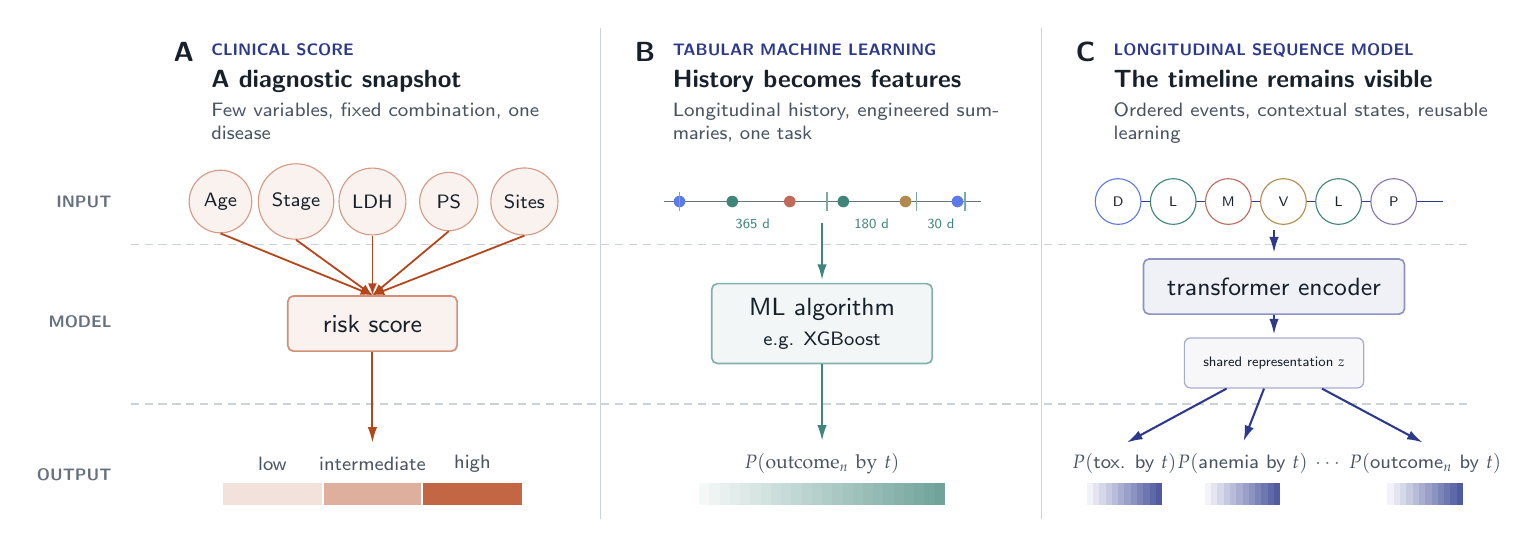
\begin{tikzpicture}[opera,x=1cm,y=1cm]
  \draw[divider] (5.55,.05)--(5.55,-6.18);
  \draw[divider] (11.15,.05)--(11.15,-6.18);

  % Shared semantic bands make the three paradigms directly comparable.
  \begin{scope}[on background layer]
    \draw[draw=OperaBorder,densely dashed,line width=.45pt] (-.42,-2.70)--(16.55,-2.70);
    \draw[draw=OperaBorder,densely dashed,line width=.45pt] (-.42,-4.72)--(16.55,-4.72);
  \end{scope}
  \node[eyebrow,anchor=east,text=OperaInkMuted] at (-.54,-2.15) {INPUT};
  \node[eyebrow,anchor=east,text=OperaInkMuted] at (-.54,-3.68) {MODEL};
  \node[eyebrow,anchor=east,text=OperaInkMuted] at (-.54,-5.62) {OUTPUT};

  % A — clinical score
  \node[panelletter,anchor=north west] at (0,0) {A};
  \node[eyebrow,anchor=north west] at (.48,-.03) {CLINICAL SCORE};
  \node[heading,anchor=north west] at (.48,-.36) {A diagnostic snapshot};
  \node[labelsmall,anchor=north west,align=left,text width=4.65cm] at (.48,-.78)
    {Few variables, fixed combination, one disease};
  \foreach \name/\x/\lab in {age/.72/Age,stage/1.68/Stage,
      ldh/2.65/LDH,ps/3.62/PS,sites/4.58/Sites}
    \node[circle,draw=OperaSienna!55,fill=OperaSienna!7,minimum size=7.4mm,
      font=\sffamily\scriptsize] (\name) at (\x,-2.15) {\lab};
  \node[stagewarm,minimum width=2.15cm,minimum height=7mm] (score) at (2.65,-3.70) {risk score};
  \foreach \name in {age,stage,ldh,ps,sites}
    \draw[-{Latex[length=1.5mm]},draw=OperaSienna,line width=.65pt]
      (\name.south)--(score.north);
  \draw[flowwarm,shorten >=1pt] (score.south)--(2.65,-5.25);
  % Clinical scores define discrete strata, not a continuous probability scale.
  \node[labelsmall] at (1.38,-5.48) {low};
  \node[labelsmall] at (2.65,-5.48) {intermediate};
  \node[labelsmall] at (3.92,-5.48) {high};
  \fill[OperaSienna!16] (.75,-6.00) rectangle (2.02,-5.72);
  \fill[OperaSienna!43] (2.02,-6.00) rectangle (3.28,-5.72);
  \fill[OperaSienna!82] (3.28,-6.00) rectangle (4.55,-5.72);
  \draw[white,line width=.8pt] (2.02,-6.00)--(2.02,-5.72);
  \draw[white,line width=.8pt] (3.28,-6.00)--(3.28,-5.72);
  %\node[captionnote,text width=4.4cm] at (2.65,-6.72)
  %  {Interpretable and portable, but most prior history is compressed away.};

  % B — tabular model
  \node[panelletter,anchor=north west] at (5.86,0) {B};
  \node[eyebrow,anchor=north west] at (6.34,-.03) {TABULAR MACHINE LEARNING};
  \node[heading,anchor=north west] at (6.34,-.36) {History becomes features};
  \node[labelsmall,anchor=north west,align=left,text width=4.55cm] at (6.34,-.78)
    {Longitudinal history, engineered summaries, one task};
  \draw[OperaInkMuted,line width=.55pt] (6.35,-2.15)--(10.38,-2.15);
  \foreach \x/\col in {6.55/OperaPeriwinkle,7.22/OperaTeal,7.95/OperaTerracotta,
      8.63/OperaTeal,9.42/OperaOchre,10.08/OperaPeriwinkle}
    \fill[\col] (\x,-2.15) circle (2.1pt);
  % One history, partitioned into look-back intervals for aggregation.
  \foreach \x in {6.55,8.42,9.56,10.18}
    \draw[draw=OperaTeal!68,line width=.65pt] (\x,-2.03)--(\x,-2.27);
  \node[font=\sffamily\tiny,text=OperaTeal] at (7.48,-2.43) {365 d};
  \node[font=\sffamily\tiny,text=OperaTeal] at (8.99,-2.43) {180 d};
  \node[font=\sffamily\tiny,text=OperaTeal] at (9.87,-2.43) {30 d};
  \node[stage,draw=OperaTeal!65,fill=OperaTeal!7,minimum width=2.80cm,
    minimum height=7mm] (ml) at (8.36,-3.70)
    {ML algorithm\\{\scriptsize e.g. XGBoost}};
  \draw[flowteal,shorten >=1pt] (8.36,-2.42)--(ml.north);
  \node[labelsmall] (prob) at (8.36,-5.48) {$P(\mathrm{outcome}_n\ \mathrm{by}\ t)$};
  \draw[flowteal,shorten >=1pt] (ml.south)--(prob.north);
  \foreach \i in {0,...,23}{
    \pgfmathsetmacro{\xa}{6.80+0.13*\i}
    \pgfmathsetmacro{\xb}{6.80+0.13*(\i+1)}
    \pgfmathtruncatemacro{\tone}{6+3*\i}
    \fill[OperaTeal!\tone] (\xa,-6.00) rectangle (\xb,-5.72);
  }
  %\node[captionnote,text width=4.4cm] at (8.36,-6.72)
  %  {A separate predictor is typically fitted for each outcome and horizon.};

  % C — sequence model
  \node[panelletter,anchor=north west] at (11.46,0) {C};
  \node[eyebrow,anchor=north west] at (11.94,-.03) {LONGITUDINAL SEQUENCE MODEL};
  \node[heading,anchor=north west] at (11.94,-.36) {The timeline remains visible};
  \node[labelsmall,anchor=north west,align=left,text width=4.75cm] at (11.94,-.78)
    {Ordered events, contextual states, reusable learning};
  \draw[OperaIndigo,line width=.65pt] (11.95,-2.15)--(16.25,-2.15);
  \foreach \x/\col/\lab in {12.12/OperaPeriwinkle/D,12.82/OperaTeal/L,
      13.52/OperaTerracotta/M,14.22/OperaOchre/V,14.92/OperaTeal/L,15.62/OperaLavender/P}
    \node[circle,draw=\col,fill=white,minimum size=5.8mm,font=\sffamily\tiny] at (\x,-2.15) {\lab};
  \draw[flowblue] (14.10,-2.51)--(14.10,-2.80);
  \node[stageblue,minimum width=3.00cm,minimum height=7mm] (enc) at (14.10,-3.23)
    {transformer encoder};
  \node[softpanel,draw=OperaIndigo!42,fill=OperaIndigo!4,
    minimum width=2.25cm,minimum height=5.5mm,font=\sffamily\tiny]
    (z) at (14.10,-4.20) {shared representation $z$};
  \draw[flowblue,shorten >=1pt] (enc.south)--(z.north);
  \node[labelsmall] (c1) at (12.20,-5.48) {$P($tox. by $t)$};
  \node[labelsmall] (c2) at (13.70,-5.48) {$P($anemia by $t)$};
  \node[font=\sffamily\scriptsize,text=OperaInkMuted] at (14.80,-5.48) {$\cdots$};
  \node[labelsmall] (cn) at (16.02,-5.48) {$P($outcome$_n$ by $t)$};
  \draw[flowblue,shorten >=1pt] (z)--(c1.north);
  \draw[flowblue,shorten >=1pt] (z)--(c2.north);
  \draw[flowblue,shorten >=1pt] (z)--(cn.north);
  % Each task emits its own continuous probability, aligned with panel B.
  \begin{scope}[shift={(11.72,0)}]
    \foreach \i in {0,...,11}{
      \pgfmathsetmacro{\xa}{0.08*\i}
      \pgfmathsetmacro{\xb}{0.08*(\i+1)}
      \pgfmathtruncatemacro{\tone}{6+7*\i}
      \fill[OperaIndigo!\tone] (\xa,-6.00) rectangle (\xb,-5.72);
    }
  \end{scope}
  \begin{scope}[shift={(13.22,0)}]
    \foreach \i in {0,...,11}{
      \pgfmathsetmacro{\xa}{0.08*\i}
      \pgfmathsetmacro{\xb}{0.08*(\i+1)}
      \pgfmathtruncatemacro{\tone}{6+7*\i}
      \fill[OperaIndigo!\tone] (\xa,-6.00) rectangle (\xb,-5.72);
    }
  \end{scope}
  \begin{scope}[shift={(15.54,0)}]
    \foreach \i in {0,...,11}{
      \pgfmathsetmacro{\xa}{0.08*\i}
      \pgfmathsetmacro{\xb}{0.08*(\i+1)}
      \pgfmathtruncatemacro{\tone}{6+7*\i}
      \fill[OperaIndigo!\tone] (\xa,-6.00) rectangle (\xb,-5.72);
    }
  \end{scope}
  %\node[captionnote,text width=4.55cm] at (14.10,-6.72)
  %  {The encoder may be pretrained; one representation can support many outcomes and horizons.};
\end{tikzpicture}
}\par\vspace{3mm}
  \resizebox{\textwidth}{!}{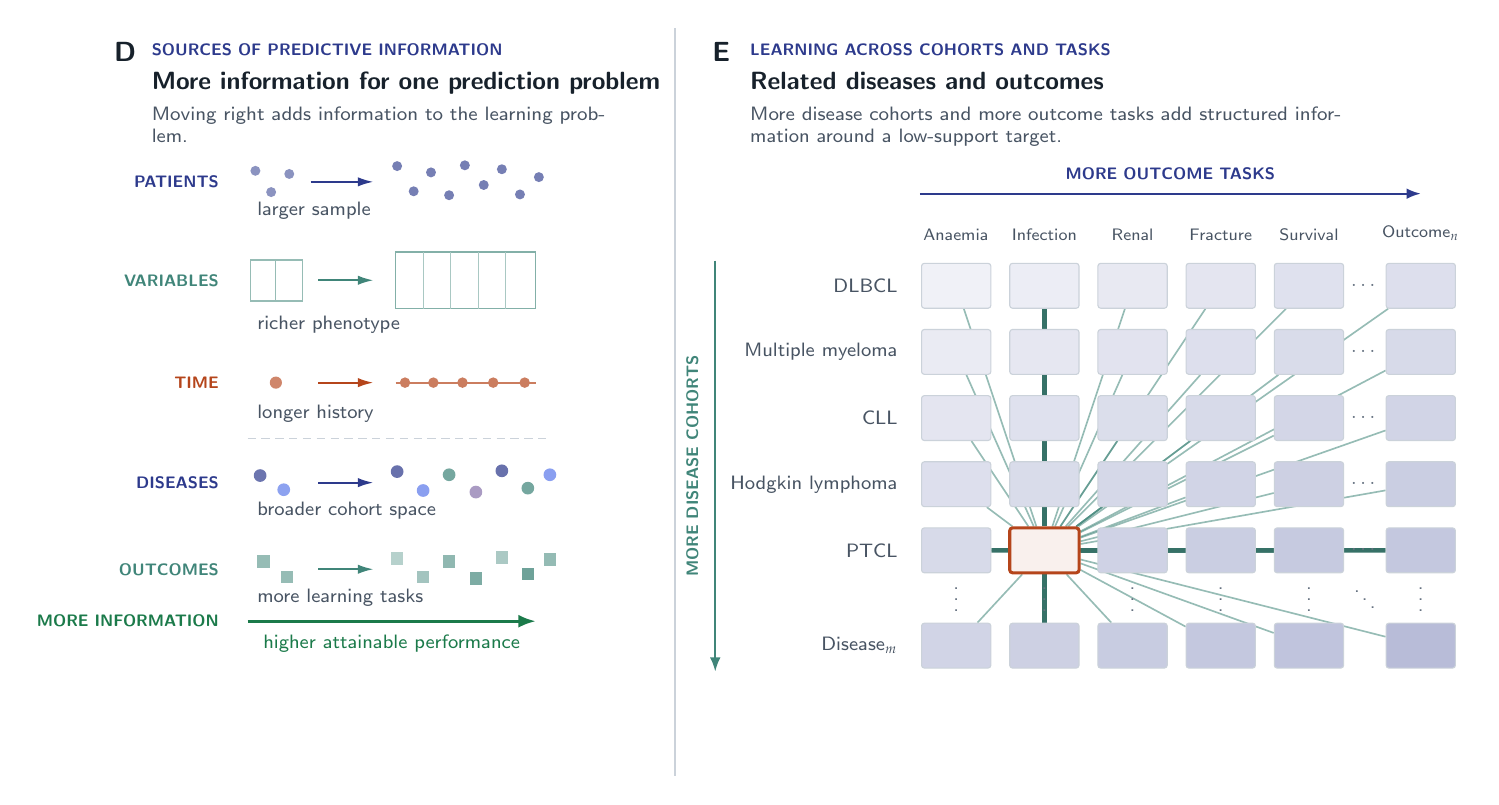
\begin{tikzpicture}[opera,x=1cm,y=1cm]
  \draw[divider] (7.25,.05)--(7.25,-9.45);

  \node[panelletter,anchor=north west] at (0,0) {D};
  \node[eyebrow,anchor=north west] at (.48,-.03) {SOURCES OF PREDICTIVE INFORMATION};
  \node[heading,anchor=north west] at (.48,-.38) {More information for one prediction problem};
  \node[labelsmall,anchor=north west,align=left,text width=5.9cm] at (.48,-.82)
    {Moving right adds information to the learning problem.};

  % Concrete before-to-after examples are easier to read than abstract axes.
  \node[eyebrow,text=OperaIndigo,anchor=east] at (1.58,-1.90) {PATIENTS};
  \foreach \x/\y in {1.92/-1.76,2.12/-2.03,2.35/-1.80}
    \fill[OperaIndigo!55] (\x,\y) circle (1.8pt);
  \draw[flowblue] (2.62,-1.90)--(3.42,-1.90);
  \foreach \x/\y in {3.72/-1.70,3.93/-2.02,4.15/-1.78,4.38/-2.07,4.58/-1.69,
      4.82/-1.94,5.05/-1.74,5.28/-2.06,5.52/-1.84}
    \fill[OperaIndigo!65] (\x,\y) circle (1.8pt);
  \node[labelsmall,anchor=west] at (1.82,-2.27) {larger sample};

  \node[eyebrow,text=OperaTeal,anchor=east] at (1.58,-3.15) {VARIABLES};
  \draw[OperaTeal!55,line width=.55pt] (1.86,-3.41) rectangle (2.52,-2.89);
  \draw[OperaTeal!55,line width=.45pt] (2.18,-3.41)--(2.18,-2.89);
  \draw[flowteal] (2.72,-3.15)--(3.42,-3.15);
  \draw[OperaTeal!65,line width=.55pt] (3.70,-3.51) rectangle (5.48,-2.79);
  \foreach \x in {4.05,4.40,4.75,5.10}\draw[OperaTeal!45,line width=.4pt] (\x,-3.51)--(\x,-2.79);
  \node[labelsmall,anchor=west] at (1.82,-3.72) {richer phenotype};

  \node[eyebrow,text=OperaSienna,anchor=east] at (1.58,-4.45) {TIME};
  \fill[OperaSienna!65] (2.18,-4.45) circle (2.2pt);
  \draw[flowwarm] (2.72,-4.45)--(3.42,-4.45);
  \draw[OperaSienna!70,line width=.65pt] (3.70,-4.45)--(5.48,-4.45);
  \foreach \x in {3.82,4.18,4.55,4.94,5.34}\fill[OperaSienna!70] (\x,-4.45) circle (1.9pt);
  \node[labelsmall,anchor=west] at (1.82,-4.85) {longer history};

  \draw[draw=OperaBorder,densely dashed,line width=.5pt] (1.82,-5.16)--(5.62,-5.16);

  \node[eyebrow,text=OperaIndigo,anchor=east] at (1.58,-5.72) {DISEASES};
  \foreach \x/\y/\col in {1.98/-5.63/OperaIndigo,2.28/-5.81/OperaPeriwinkle}
    \fill[\col!70] (\x,\y) circle (2.3pt);
  \draw[flowblue] (2.72,-5.72)--(3.42,-5.72);
  \foreach \x/\y/\col in {3.72/-5.58/OperaIndigo,4.05/-5.82/OperaPeriwinkle,
      4.38/-5.62/OperaTeal,4.72/-5.84/OperaLavender,5.05/-5.57/OperaIndigo,
      5.38/-5.79/OperaTeal,5.66/-5.62/OperaPeriwinkle}
    \fill[\col!72] (\x,\y) circle (2.3pt);
  \node[labelsmall,anchor=west] at (1.82,-6.08) {broader cohort space};

  \node[eyebrow,text=OperaTeal,anchor=east] at (1.58,-6.82) {OUTCOMES};
  \foreach \x/\y in {2.02/-6.72,2.32/-6.92}
    \fill[OperaTeal!55] (\x-.08,\y-.08) rectangle (\x+.08,\y+.08);
  \draw[flowteal] (2.72,-6.82)--(3.42,-6.82);
  \foreach \x/\y/\tone in {3.72/-6.68/38,4.05/-6.92/48,4.38/-6.72/58,
      4.72/-6.94/68,5.05/-6.67/44,5.38/-6.88/76,5.66/-6.70/56}
    \fill[OperaTeal!\tone] (\x-.08,\y-.08) rectangle (\x+.08,\y+.08);
  \node[labelsmall,anchor=west] at (1.82,-7.18) {more learning tasks};
  \node[eyebrow,text=OperaGreen,anchor=east] at (1.58,-7.48) {MORE INFORMATION};
  \draw[-{Latex[length=2.2mm]},draw=OperaGreen,line width=1pt] (1.82,-7.48)--(5.48,-7.48);
  \node[labelsmall,text=OperaGreen] at (3.65,-7.76)
    {higher attainable performance};

  \node[panelletter,anchor=north west] at (7.60,0) {E};
  \node[eyebrow,anchor=north west] at (8.08,-.03) {LEARNING ACROSS COHORTS AND TASKS};
  \node[heading,anchor=north west] at (8.08,-.38) {Related diseases and outcomes};
  \node[labelsmall,anchor=north west,align=left,text width=7.6cm] at (8.08,-.82)
    {More disease cohorts and more outcome tasks add structured information around a low-support target.};

  % Separate the axis/title and matrix from the two-line panel introduction.
  \begin{scope}[yshift=-5mm]
  % Keep the axis title separate from the column labels and first row.
  \draw[-{Latex[length=1.8mm]},draw=OperaIndigo,line width=.75pt]
    (10.36,-1.55)--(16.72,-1.55);
  \node[eyebrow,text=OperaIndigo] at (13.54,-1.30) {MORE OUTCOME TASKS};

  \foreach \r/\disease in {0/DLBCL,1/Multiple myeloma,2/CLL,3/Hodgkin lymphoma,4/PTCL}
    \node[labelsmall,anchor=east] at (10.20,-2.72-.84*\r) {\disease};
  \draw[-{Latex[length=1.8mm]},draw=OperaTeal,line width=.75pt]
    (7.76,-2.40)--(7.76,-7.62);
  \node[eyebrow,text=OperaTeal,rotate=90] at (7.47,-5.01) {MORE DISEASE COHORTS};
  \foreach \col/\outcome in {0/Anaemia,1/Infection,2/Renal,3/Fracture,4/Survival}
    \node[font=\sffamily\fontsize{6.2}{7}\selectfont,text=OperaInkSecondary,
      align=center,text width=1.05cm,anchor=south] at (10.82+1.12*\col,-2.27) {\outcome};
  \node[font=\sffamily\fontsize{6.2}{7}\selectfont,text=OperaInkSecondary,
    align=center,text width=1.05cm,anchor=south] at (16.72,-2.27) {Outcome$_n$};
  \foreach \r in {0,...,4}{\foreach \col in {0,...,4}{
    \pgfmathtruncatemacro{\tone}{7+3*\r+2*\col}
    \node[rounded corners=.35mm,draw=OperaBorder,fill=OperaIndigo!\tone,
      minimum width=8.8mm,minimum height=5.7mm] (m\r\col)
      at (10.82+1.12*\col,-2.72-.84*\r) {};
  }}
  \foreach \r in {0,...,4}{
    \node[font=\sffamily\scriptsize,text=OperaInkMuted]
      at (16.01,-2.72-.84*\r) {$\cdots$};
  }
  \foreach \r in {0,...,4}{
    \pgfmathtruncatemacro{\tone}{16+3*\r}
    \node[rounded corners=.35mm,draw=OperaBorder,fill=OperaIndigo!\tone,
      minimum width=8.8mm,minimum height=5.7mm] (mn\r) at (16.72,-2.72-.84*\r) {};
  }
  \foreach \x in {10.82,11.94,13.06,14.18,15.30,16.72}{
    \node[font=\sffamily\scriptsize,text=OperaInkMuted] at (\x,-6.60) {$\vdots$};
  }
  \node[font=\sffamily\scriptsize,text=OperaInkMuted] at (16.01,-6.60) {$\ddots$};
  \node[labelsmall,anchor=east] at (10.20,-7.29) {Disease$_m$};
  \foreach \col in {0,...,4}{
    \pgfmathtruncatemacro{\tone}{22+2*\col}
    \node[rounded corners=.35mm,draw=OperaBorder,fill=OperaIndigo!\tone,
      minimum width=8.8mm,minimum height=5.7mm] (mm\col)
      at (10.82+1.12*\col,-7.29) {};
  }
  \node[rounded corners=.35mm,draw=OperaBorder,fill=OperaIndigo!34,
    minimum width=8.8mm,minimum height=5.7mm] (mmn) at (16.72,-7.29) {};
  \node[rounded corners=.35mm,draw=OperaSienna,line width=1.1pt,fill=OperaSienna!8,
    minimum width=8.8mm,minimum height=5.7mm] (target) at (11.94,-6.08) {};
  % Every training cell is connected; most links recede behind the emphasized
  % same-outcome and same-disease borrowing paths.
  \begin{scope}[on background layer]
    \foreach \r in {0,...,4}{\foreach \col in {0,...,4}{
      \draw[draw=OperaTeal,opacity=.55,line width=.6pt] (m\r\col)--(target);
    }}
    \foreach \r in {0,...,4}{
      \draw[draw=OperaTeal,opacity=.55,line width=.6pt] (mn\r)--(target);
    }
    \foreach \col in {0,...,4}{
      \draw[draw=OperaTeal,opacity=.55,line width=.6pt] (mm\col)--(target);
    }
    \draw[draw=OperaTeal,opacity=.55,line width=.6pt] (mmn)--(target);
    \foreach \r in {0,...,3}{
      \draw[draw=OperaTeal!85!black,opacity=1,line width=1.6pt] (m\r1)--(target);
    }
    \foreach \col in {0,2,3,4}{
      \draw[draw=OperaTeal!85!black,opacity=1,line width=1.6pt] (m4\col)--(target);
    }
    % The last disease (same outcome) and last outcome (same disease) borrow too.
    \draw[draw=OperaTeal!85!black,opacity=1,line width=1.6pt] (mm1)--(target);
    \draw[draw=OperaTeal!85!black,opacity=1,line width=1.6pt] (mn4)--(target);
  \end{scope}
  \end{scope}
\end{tikzpicture}
}
  \caption{\textbf{Approaches to risk prediction and the information each
  can use.} Top, three approaches for haematological risk prediction.
  \textbf{A}, clinical risk scores combine a small diagnostic snapshot with a
  fixed rule into broad risk strata. \textbf{B}, classical machine learning
  uses a wider history, aggregated over time into a task-specific feature
  table. \textbf{C}, a longitudinal sequence model reads the ordered clinical
  events and can share one patient representation across outcomes. Its encoder may be pretrained locally or at nation scale. Bottom, sources of additional
  predictive information. \textbf{D}, conventional scaling adds patients,
  variables or observations to an isolated prediction problem. \textbf{E},
  joint modelling can also draw on related diseases (rows) and outcomes
  (columns), although breadth need not improve every target. Sharing uses
  training data only, through a common encoder and readout. It transfers no future information and does not assume diseases or outcomes are
  exchangeable. The panels describe the information available to each kind of
  predictor, not the exact structure of every score or tabular model.}
  \label{fig:paradigms}
\end{figure}



\clearpage
\section*{Methods}

\subsection*{Data and study population}
DALY-CARE covers all adult Danish residents with a lymphoid cancer or related
diagnosis registered since 2002 \citep{brieghel2025dalycare}, linking the
national patient, prescription, hospital medication, laboratory, cancer and
cause-of-death registers with the clinical quality registries for lymphoma,
myeloma and chronic lymphocytic leukaemia. The sequence models read the
national patient register (diagnoses, procedures and contact attributes),
pathology codes, redeemed prescriptions, hospital-administered medication,
laboratory results, sex and date of birth. The cancer and cause-of-death registers and the quality registries were used only to define the cohort,
outcomes and benchmarks. Records were converted to a common event format with
ehr2meds (Supplementary Methods), and \cref{fig:model-inputs} shows what each source contributes. Electronic health record data, available for two of
five regions, were not used. We included adults who
started first-line treatment for a lymphoid or plasma-cell malignancy. The start of treatment was the index date and the single prediction time. Patients
were assigned to one of 24 subtypes in 10 groups from diagnoses recorded up to
14 days after the index date, or up to 90 days for late-coded diagnoses, with a
sensitivity analysis excluding the latter. Treatment lines, subtype rules and
data sources are detailed in the Supplementary Methods. The study was approved
by the Danish Health Data Authority (P-2020-561) and the National Ethics
Committee (1804410).

\subsection*{Intended use}
The models are intended for the haematologist at the start of first-line
treatment for a lymphoid cancer. For each patient they estimate the risk of
every outcome in the panel over the following two years, from the records
available at that point, as a basis for planning monitoring, prophylaxis and
supportive care, for discussing prognosis with the patient and for identifying
candidates for trials. They are not intended to choose between treatment
regimens, which would require predictions conditional on the regimen.

\subsection*{Prediction time and temporal validation}
Inputs were restricted to information recorded before the index date.
Patients treated until the end of 2021 formed the training set, those treated in
2022 the tuning set used for every model and checkpoint choice, and those
treated from 2023 the test set, analysed once after all decisions had been
fixed. Self-supervised pretraining used only events before 1 January 2022. Some test patients therefore contributed earlier history to pretraining, but no
outcome after 2021 was used in any training.

\subsection*{Outcomes}
The 69 outcomes span disease course (second-line treatment, treatment failure,
transformation, new malignancy and death), infection, haematological, renal,
hepatic and metabolic toxicity, cardiovascular events and acute care, each
predicted at 30, 60, 90, 180, 365 and 730 days. Laboratory outcomes use grading
thresholds aligned with, but not identical to, the Common Terminology Criteria
for Adverse Events, adjusted for abnormal pre-treatment values
\citep{nci2025ctcae}, and infection is partly captured through antimicrobial treatment. A patient contributed to an outcome only if it was
ascertainable for them, death competed with every non-fatal outcome, and the
panel was selected from 87 candidates using training and tuning data only.
For presentation, outcomes are grouped into clinical domains (for example
infection, renal injury, or sodium and potassium), and the domains play no part in training. Definitions and risk sets are in the Supplementary Methods.

\subsection*{Models}
Every neural model shares one architecture: a causal transformer encoder,
building on CORE-BEHRT \citep{odgaard2024core}, pretrained to predict the next
event in each patient's chronological history of diagnoses, procedures,
pathology, medications, laboratory results and hospital contacts, followed by
a linear head that
produces outcome-specific hazards with death as a competing risk
\citep{gensheimer2019nnetsurvival,lee2018deephit}. Supervised training
minimised a cross-entropy at each horizon over patients with known status,
with the grade variants of one laboratory finding (grade $\geq$2 and
$\geq$3) weighted together as one endpoint, so that the 69 outcomes counted as
52 endpoints.
The four supervision scopes differed only in which cells of the
disease-by-outcome grid (one outcome in one disease) provided labels
(\cref{fig:supervision-grid}): a specialist learned one cell, a disease-pooled
model one outcome across all diseases, an outcome-pooled model all outcomes in
one disease, and the joint model every cell. All were trained with the same
encoder initialisation and optimiser for up to 30 epochs, stopping after five
epochs without improvement in tuning loss, and kept the tuning-best checkpoint. The routed model used the joint
model's labels but let each prediction weight low-rank adapters owned by
individual diseases and outcomes \citep{ma2018mmoe,houlsby2019adapters}, with its configuration chosen on the tuning set. Because the router is the only model
told the patient's disease, three controls separate what it adds: the joint
model with a learned disease embedding (identity alone), and routers restricted
to the patient's own disease adapter or the target's own outcome adapter
(specific capacity without borrowing). As a control for pretraining
itself, one joint model was trained from a randomly initialised encoder of the
same architecture. Encoder, objective and router are
specified in the Supplementary Methods.

\subsection*{National pretraining and local adaptation}
We also initialised the joint and routed models from the national encoder of
the PHAIR project, pretrained on the registers of the entire Danish population
with the same 1 January 2022 cutoff for 10 epochs \placeholder{number of individuals and events, reference}, used either directly or after 20 epochs of
continued pretraining on our records (local adaptation). This gave the same exposure to our records as the local encoder, which was pretrained for 20 epochs with the
validation-best checkpoint retained. For the national encoder, our patients'
records were taken from the national data extract and tokenised with its own
vocabulary and preprocessing, so that it read them in the form it was trained on. Outcomes, cohort membership and splits were unchanged.
Downstream training was identical for the local, national and adapted national
encoders, so the comparisons concern the encoders as delivered, which may also
differ in population, coding and training budget.

\subsection*{Benchmarks}
For each cell and horizon we trained XGBoost \citep{chen2016xgboost} and
ridge-penalised logistic regression on features from the pipeline of our earlier
DLBCL study \citep{werling2026dlbcl}: history summaries over three windows
before the index date, built with timeseriesflattener
\citep{bernstorff2023tsflattener}, with quality-registry variables and
registry-recorded adverse events removed so that tabular and sequence models
received the same information. To separate
the value of pooling from the value of the neural model, we also trained one
XGBoost per outcome across all diseases. This is the tabular counterpart of the disease-pooled model and, like it, is not told the patient's disease.
Clinical quality-registry variables such as performance status, stage,
lactate dehydrogenase and cytogenetics were among the strongest predictors in
the earlier study but are not part of the records the sequence models read. As a reference, we therefore also trained XGBoost for each cell with these
variables added. Hyperparameters, including the setting of the earlier study,
were chosen on tuning-set log loss, and no model was class-reweighted.

\subsection*{Clinical prognostic indices}
The quality registries record which prognostic index was scored at diagnosis
and its risk category. We compared the joint model with every index recorded
for at least 50 patients of a subtype, in the patients who had it, for
two-year treatment failure, and each index used in several subtypes also
across all of them, since the IPI, for instance, is applied to many rare lymphomas for which no specific score exists. In DLBCL we also computed the NCCN-IPI from its
recorded components \citep{zhou2014nccnipi}. Model risk groups were defined on
the tuning set to mirror the index at both ends: the low-risk group was the
largest whose observed risk did not exceed that of the index's low-risk
category, the high-risk group flagged the same proportion of patients without
the event as the index's high-risk category (equal specificity), and patients
between them were divided in the proportions of the index's intermediate
categories. The comparison then asks how many more events the model's
high-risk group captures at the index's false-alarm rate, and how many patients
it can place at low risk without raising their risk. The observed risk in the model's highest-risk 5\% and 10\% shows what it identifies beyond the index's
top category. Details and a size-matched sensitivity analysis are in the
Supplementary Methods.

\subsection*{Evaluation}
Discrimination was measured by the time-dependent AUC and accuracy by the
index of prediction accuracy (IPA), one minus the ratio of a model's Brier
score to that of the observed event rate \citep{kattan2018ipa}, both for the
predicted cumulative incidence and weighted by the inverse probability of
censoring, with deaths from other causes counted as non-events
\citep{blanche2013competingauc,gerds2006brier}. Calibration was measured by the calibration slope and calibration-in-the-large. The AUC was the primary metric and IPA the
key secondary, with Brier score differences reported alongside. One year is the main horizon, and all six are reported. Models were compared on identical
patients: patients were resampled 1,000 times within each disease, and the
same resamples were reused across models, outcomes and horizons. Each model was
trained once, so intervals reflect uncertainty from the test patients only.
Effects across cells were summarised with a hierarchical model with crossed
disease and outcome effects, a smooth curve in the number of training events
and weakly informative priors, always alongside the raw cell estimates. Every disease weighed equally and, within a disease, every endpoint. Because training
support varies naturally, these curves describe association rather than the
effect of fewer labels. A model was called better when the 95\% interval of
its pooled gain excluded zero and the probability of a gain larger than a
practical margin of \placeholder{0.01} was at least 0.95, equivalent when the
interval lay within the margin, and inconclusive otherwise. We also report each
model at fixed decision points. For every model, cell and horizon, a threshold
was chosen on that model's tuning predictions and applied unchanged to test
patients with known status. The thresholds flagged as many patients as the
tuning event rate, maximised Youden's index or the Matthews correlation
coefficient (MCC), or reached a tuning specificity of 80\%, 90\% or 95\%. At
each, we report the confusion matrix, sensitivity, specificity, positive and
negative predictive values and MCC, with paired intervals from the same
resamples. These decision-point metrics are secondary and descriptive. Groups of cells
for secondary analyses (where joint learning hurt, and the best narrower model
for each cell) were defined on the tuning set. Subgroups used only information
available at the index date. Statistical details are in the
Supplementary Methods. Because the registries are national and the models were
trained on the whole country, we report performance by the region in which each
patient had most of their pre-treatment contacts rather than holding regions out.
Reporting follows TRIPOD+AI \citep{collins2024tripodai}.

\FloatBarrier
% Fill-in contract and figure rationale: RESULTS_OUTLINE.md and FIGURE_PLACEMENT.md.
\section*{Results}
\subsection*{Who was studied, and what was predicted?}
Of 78,668 adults in DALY-CARE with a lymphoid cancer or related diagnosis,
37,531 started first-line treatment and were included (\cref{fig:cohort-flow}):
29,105 in the training period (to 2021), 1,980 in the tuning year (2022) and
6,446 in the test period (from 2023). \placeholder{Median age, sex and the
largest disease groups (Table~1).} Of the 24 diseases and 69 outcomes,
\placeholder{N} cells had enough test events to be
evaluated at one year. Event rates ranged from \placeholder{range}, and
\placeholder{N} cells had fewer than 20 events to train on
(\cref{fig:supp-coverage,fig:supp-support}).

% The checked-in table1.tex is a historical layout, not current approved data.
\IfFileExists{tables/table1_current_approved.tex}{
  \input{tables/table1_current_approved}
}{
  \IfFileExists{tables/table1_current_review.tex}{
    \noindent\placeholder{Current server-derived Table 1: supervisor review pending.}
    % Generated by opera.run.format_table1_release from export sha256 b19cf510d55a662b8e42fbfe9f4a494712762273b4e8ace6e5c97c5d2038bab6 (disclosure policy: primary-only).
% Do not edit values by hand; regenerate from the reviewed export.
\begin{table*}[p]
\centering
\caption{\textbf{Baseline characteristics at first-line treatment.} One record per patient at the shared first-line index, by temporal split. Values are $n$ (\%) or median (IQR).}
\label{tab:characteristics}
\footnotesize
\setlength{\tabcolsep}{4pt}
\renewcommand{\arraystretch}{1.05}
\begin{tabularx}{\textwidth}{@{}Xrrrr@{}}
\toprule
Characteristic & Overall & Training & Tuning & Test \\
 & {\footnotesize\itshape All years} & {\footnotesize\itshape Through 2021} & {\footnotesize\itshape 2022} & {\footnotesize\itshape From 2023} \\
& {\footnotesize $n$ = 37,531} & {\footnotesize $n$ = 29,105} & {\footnotesize $n$ = 1,980} & {\footnotesize $n$ = 6,446} \\
\midrule
\addlinespace
\multicolumn{5}{@{}l}{\sffamily\bfseries Demographics}\\
Age at treatment, years & 69 (60–77) & 69 (59–77) & 71 (61–78) & 72 (62–79) \\
Age $\geq$70 years & 18,108 (48.2\%) & 13,470 (46.3\%) & 1,065 (53.8\%) & 3,573 (55.4\%) \\
Female & 15,665 (41.7\%) & 12,195 (41.9\%) & 808 (40.8\%) & 2,662 (41.3\%) \\
Year of treatment & 2016 (2010–2021) & 2014 (2009–2018) & 2022 (2022–2022) & 2024 (2023–2025) \\
\addlinespace
\multicolumn{5}{@{}l}{\sffamily\bfseries Disease}\\
\multicolumn{5}{@{}l}{Disease group and subtype}\\
\quad \textbf{Large B-cell lymphomas} & 10,388 (27.7\%) & 8,356 (28.7\%) & 500 (25.3\%) & 1,532 (23.8\%) \\
\qquad Diffuse large B-cell (DLBCL) & 9,935 (26.5\%) & 7,996 (27.5\%) & 476 (24.0\%) & 1,463 (22.7\%) \\
\qquad Transformed follicular (tFL)$^{\dagger}$ & 264 (0.7\%) & 210 (0.7\%) & 10 (0.5\%) & 44 (0.7\%) \\
\qquad Richter transformation (RT)$^{\dagger}$ & 189 (0.5\%) & 150 (0.5\%) & 14 (0.7\%) & 25 (0.4\%) \\
\quad \textbf{Burkitt and lymphoblastic lymphomas} & 1,365 (3.6\%) & 1,074 (3.7\%) & 86 (4.3\%) & 205 (3.2\%) \\
\qquad Lymphoblastic (LBL)$^{\dagger}$ & 1,073 (2.9\%) & 838 (2.9\%) & 71 (3.6\%) & 164 (2.5\%) \\
\qquad Burkitt (BL) & 292 (0.8\%) & 236 (0.8\%) & 15 (0.8\%) & 41 (0.6\%) \\
\quad \textbf{Mantle-cell lymphoma (MCL)} & 1,467 (3.9\%) & 1,117 (3.8\%) & 86 (4.3\%) & 264 (4.1\%) \\
\quad \textbf{Indolent B-cell lymphomas} & 5,414 (14.4\%) & 3,891 (13.4\%) & 308 (15.6\%) & 1,215 (18.8\%) \\
\qquad Follicular (FL) & 2,929 (7.8\%) & 2,242 (7.7\%) & 152 (7.7\%) & 535 (8.3\%) \\
\qquad Lymphoplasmacytic (LPL) & 1,580 (4.2\%) & 1,168 (4.0\%) & 101 (5.1\%) & 311 (4.8\%) \\
\qquad Extranodal marginal-zone (EMZL) & 500 (1.3\%) & 318 (1.1\%) & 32 (1.6\%) & 150 (2.3\%) \\
\qquad Unspecified B-cell (BCL)$^{\dagger}$ & 234 (0.6\%) & 87 (0.3\%) & 21 (1.1\%) & 126 (2.0\%) \\
\qquad Splenic marginal-zone (SMZL) & 144 (0.4\%) & 71 (0.2\%) & $<$5 & 71 (1.1\%) \\
\qquad Nodal marginal-zone (NMZL)$^{\dagger}$ & 27 (0.1\%) & 5 (0.0\%) &  & 22 (0.3\%) \\
\quad \textbf{CLL and SLL} & 5,183 (13.8\%) & 4,102 (14.1\%) & 254 (12.8\%) & 827 (12.8\%) \\
\qquad Chronic lymphocytic leukaemia (CLL) & 4,091 (10.9\%) & 3,230 (11.1\%) & 195 (9.8\%) & 666 (10.3\%) \\
\qquad Small lymphocytic lymphoma (SLL) & 1,092 (2.9\%) & 872 (3.0\%) & 59 (3.0\%) & 161 (2.5\%) \\
\quad \textbf{Hairy-cell leukaemia (HCL)$^{\dagger}$} & 424 (1.1\%) & 295 (1.0\%) & 29 (1.5\%) & 100 (1.6\%) \\
\quad \textbf{Hodgkin lymphoma (HL)} & 2,636 (7.0\%) & 2,072 (7.1\%) & 141 (7.1\%) & 423 (6.6\%) \\
\quad \textbf{T-cell lymphomas} & 1,646 (4.4\%) & 1,287 (4.4\%) & 70 (3.5\%) & 289 (4.5\%) \\
\qquad Peripheral T-cell, NOS (PTCL) & 521 (1.4\%) & 443 (1.5\%) & 18 (0.9\%) & 60 (0.9\%) \\
\qquad Angioimmunoblastic (AITL) & 484 (1.3\%) & 352 (1.2\%) & 26 (1.3\%) & 106 (1.6\%) \\
\qquad Anaplastic large-cell (ALCL)$^{\dagger}$ & 417 (1.1\%) & 343 (1.2\%) & 11 (0.6\%) & 63 (1.0\%) \\
\qquad Unspecified T-cell (TCL)$^{\dagger}$ & 224 (0.6\%) & 149 (0.5\%) & 15 (0.8\%) & 60 (0.9\%) \\
\quad \textbf{Plasma-cell neoplasms} & 8,962 (23.9\%) & 6,889 (23.7\%) & 499 (25.2\%) & 1,574 (24.4\%) \\
\qquad Multiple myeloma (MM) & 8,630 (23.0\%) & 6,656 (22.9\%) & 470 (23.7\%) & 1,504 (23.3\%) \\
\qquad Plasma-cell leukaemia (PCL)$^{\dagger}$ & 201 (0.5\%) & 143 (0.5\%) & 20 (1.0\%) & 38 (0.6\%) \\
\qquad Solitary plasmacytoma$^{\dagger}$ & 131 (0.3\%) & 90 (0.3\%) & 9 (0.5\%) & 32 (0.5\%) \\
\quad \textbf{Amyloidosis} & 46 (0.1\%) & 22 (0.1\%) & 7 (0.4\%) & 17 (0.3\%) \\
\addlinespace
\multicolumn{5}{@{}l}{\sffamily\bfseries Pre-index history}\\
Recorded history, years & 13.9 (8.2–18.9) & 11.6 (6.9–15.8) & 20.2 (19.5–20.6) & 22.0 (21.0–23.0) \\
Recorded events & 886 (416–1,819) & 695 (341–1,353) & 2,213 (1,322–3,575) & 1,922 (1,095–3,318) \\
Distinct diagnoses & 21 (13–32) & 20 (12–30) & 24 (15–37) & 25 (15–38) \\
Distinct medications & 21 (12–34) & 19 (10–30) & 32 (21–46) & 34 (22–49) \\
Laboratory results & 197 (0–487) & 119 (0–349) & 484 (276–801) & 524 (295–881) \\
Days with hospital contact & 19 (10–35) & 16 (9–27) & 37 (22–61) & 42 (24–70) \\
Distinct contact specialties & 8 (5–11) & 7 (5–9) & 10 (8–13) & 11 (8–14) \\
Days from last record to treatment & 2 (1–5) & 2 (1–5) & 2 (1–4) & 2 (1–4) \\
\multicolumn{5}{@{}l}{Region (most contacts)}\\
\quad North Denmark & 3,977 (11.4\%) & 3,081 (11.6\%) & 207 (10.6\%) & 689 (10.8\%) \\
\quad Central Denmark & 6,189 (17.7\%) & 4,291 (16.2\%) & 455 (23.2\%) & 1,443 (22.5\%) \\
\quad Southern Denmark & 8,908 (25.5\%) & 7,072 (26.7\%) & 442 (22.5\%) & 1,394 (21.8\%) \\
\quad Capital Region & 11,046 (31.7\%) & 8,615 (32.5\%) & 560 (28.5\%) & 1,871 (29.2\%) \\
\quad Zealand & 4,776 (13.7\%) & 3,470 (13.1\%) & 298 (15.2\%) & 1,008 (15.7\%) \\
\addlinespace
\multicolumn{5}{@{}l}{\sffamily\bfseries Follow-up}\\
Follow-up, years & 4.1 (1.4–8.6) & 5.8 (2.1–10.1) & 3.5 (3.2–3.8) & 1.4 (0.6–2.2) \\
Died during follow-up & 18,847 (50.2\%) & 17,378 (59.7\%) & 539 (27.2\%) & 930 (14.4\%) \\
Reverse Kaplan--Meier follow-up, years & 9.1 (4.4–14.5) & 11.4 (7.7–16.1) & 3.7 (3.4–4.0) & 1.6 (0.8–2.4) \\
\bottomrule
\end{tabularx}
\par\vspace{1mm}{\scriptsize Counts of 1--4 are shown as $<$5. Percentages use patients with a recorded value; history summaries use records before the index date.}
\par{\scriptsize $^{\dagger}$No dedicated, externally validated prognostic index; the prespecified stratum of subtypes without an index (Supplementary \cref{tab:index-availability}).}
\end{table*}

  }{
    % Generated by opera.run.format_table1_release from export sha256 layout (no data) (disclosure policy: targeted).
% Do not edit values by hand; regenerate from the reviewed export.
\begin{table*}[p]
\centering
\caption{\textbf{Baseline characteristics at first-line treatment.} Layout preview: every value (·) awaits the reviewed server export. One record per patient at the shared first-line index, by temporal split.}
\label{tab:characteristics}
\footnotesize
\setlength{\tabcolsep}{5pt}
\renewcommand{\arraystretch}{1.05}
\begin{tabularx}{\textwidth}{@{}Xrrrr@{}}
\toprule
Characteristic & Overall & Training & Tuning & Test \\
 & {\footnotesize\itshape All years} & {\footnotesize\itshape Through 2021} & {\footnotesize\itshape 2022} & {\footnotesize\itshape From 2023} \\
& {\footnotesize $n$ = ·} & {\footnotesize $n$ = ·} & {\footnotesize $n$ = ·} & {\footnotesize $n$ = ·} \\
\midrule
\addlinespace
\multicolumn{5}{@{}l}{\sffamily\bfseries Demographics}\\
Age at treatment, years, median (IQR) & · & · & · & · \\
Age $\geq$70 years, $n$ (\%) & · & · & · & · \\
Female, $n$ (\%) & · & · & · & · \\
Year of treatment, median (IQR) & · & · & · & · \\
\addlinespace
\multicolumn{5}{@{}l}{\sffamily\bfseries Disease}\\
\multicolumn{5}{@{}l}{Disease group and subtype, $n$ (\%)}\\
\quad \textbf{DLBCL and related aggressive B-cell lymphomas} & · & · & · & · \\
\qquad Diffuse large B-cell lymphoma (DLBCL) & · & · & · & · \\
\qquad Richter transformation (RT)$^{\dagger}$ & · & · & · & · \\
\qquad Transformed follicular lymphoma (tFL)$^{\dagger}$ & · & · & · & · \\
\quad \textbf{Burkitt and lymphoblastic lymphoma} & · & · & · & · \\
\qquad Burkitt lymphoma (BL) & · & · & · & · \\
\qquad Lymphoblastic lymphoma (LBL)$^{\dagger}$ & · & · & · & · \\
\quad \textbf{Mantle-cell lymphoma (MCL)} & · & · & · & · \\
\quad \textbf{Indolent B-cell non-Hodgkin lymphoma} & · & · & · & · \\
\qquad B-cell lymphoma, unspecified (BCL)$^{\dagger}$ & · & · & · & · \\
\qquad Extranodal marginal-zone lymphoma (EMZL) & · & · & · & · \\
\qquad Follicular lymphoma (FL) & · & · & · & · \\
\qquad Lymphoplasmacytic lymphoma (LPL) & · & · & · & · \\
\qquad Nodal marginal-zone lymphoma (NMZL)$^{\dagger}$ & · & · & · & · \\
\qquad Splenic marginal-zone lymphoma (SMZL) & · & · & · & · \\
\quad \textbf{CLL and small lymphocytic lymphoma} & · & · & · & · \\
\qquad Chronic lymphocytic leukaemia (CLL) & · & · & · & · \\
\qquad Small lymphocytic lymphoma (SLL) & · & · & · & · \\
\quad \textbf{Hairy-cell leukaemia (HCL)$^{\dagger}$} & · & · & · & · \\
\quad \textbf{Hodgkin lymphoma (HL)} & · & · & · & · \\
\quad \textbf{T-cell non-Hodgkin lymphoma} & · & · & · & · \\
\qquad Anaplastic large-cell lymphoma (ALCL)$^{\dagger}$ & · & · & · & · \\
\qquad Angioimmunoblastic T-cell lymphoma (AITL) & · & · & · & · \\
\qquad Peripheral T-cell lymphoma, NOS (PTCL) & · & · & · & · \\
\qquad T-cell lymphoma, unspecified (TCL)$^{\dagger}$ & · & · & · & · \\
\quad \textbf{Myeloma and other plasma-cell neoplasms} & · & · & · & · \\
\qquad Multiple myeloma (MM) & · & · & · & · \\
\qquad Plasma-cell leukaemia (PCL)$^{\dagger}$ & · & · & · & · \\
\qquad Solitary plasmacytoma$^{\dagger}$ & · & · & · & · \\
\quad \textbf{Amyloidosis} & · & · & · & · \\
\addlinespace
\multicolumn{5}{@{}l}{\sffamily\bfseries Pre-index history}\\
Recorded history, years, median (IQR) & · & · & · & · \\
Recorded events, median (IQR) & · & · & · & · \\
Distinct diagnoses, median (IQR) & · & · & · & · \\
Distinct medications, median (IQR) & · & · & · & · \\
Laboratory results, median (IQR) & · & · & · & · \\
Days with hospital contact, median (IQR) & · & · & · & · \\
\multicolumn{5}{@{}l}{Region (most contacts), $n$ (\%)}\\
\quad Hovedstaden & · & · & · & · \\
\quad Midtjylland & · & · & · & · \\
\quad Nordjylland & · & · & · & · \\
\quad Sjælland & · & · & · & · \\
\quad Syddanmark & · & · & · & · \\
\addlinespace
\multicolumn{5}{@{}l}{\sffamily\bfseries Follow-up}\\
Follow-up, years, median (IQR) & · & · & · & · \\
Died during follow-up, $n$ (\%) & · & · & · & · \\
\bottomrule
\end{tabularx}

\par{\scriptsize $^{\dagger}$No dedicated, externally validated prognostic index; the prespecified stratum of subtypes without an index (Supplementary \cref{tab:index-availability}).}
\end{table*}

  }
}

\FloatBarrier
\subsection*{Does one joint model outperform current approaches?}
\placeholder{The joint model had a higher one-year AUC than per-task XGBoost in
X of Y disease--outcome cells (median gain Z, IQR), than XGBoost given the
quality-registry variables in X of Y, and than the specialist trained on each
cell alone in X of Y} (\cref{fig:headline}A--B). \placeholder{Its median gain
over XGBoost was positive / not at every horizon from 30 days to two years}
(\cref{fig:headline}D) \placeholder{and did / did not differ with the number of
events recorded before treatment} (\cref{fig:headline}E). \placeholder{At the
specificity of each clinical index's high-risk category, the model's high-risk
group contained X to Y percentage points more of the patients with the event}
(\cref{fig:headline}C).

\begin{figure}[H]
  \resultfigure{fig_headline}{Joint model versus reference methods}
    {Gains over each reference per cell, against XGBoost per cell, against the
    clinical indices, across horizons and by recorded history.}
  \caption{\textbf{Performance of the joint model relative to reference
  methods.} \textbf{A}, One-year AUC gain of the joint model over each
  reference, one point per disease--outcome cell with enough test events. Diamonds show medians, bars interquartile ranges, and the figures on the right the share of cells in which the joint model was better. \textbf{B}, One-year AUC of the joint model
  against per-task XGBoost in each cell, with point size reflecting training events.
  \textbf{C}, Share of patients with the event placed in the high-risk group by
  each clinical index and by the model at the index's specificity (cutoffs
  fixed on tuning data). \textbf{D}, Median AUC gain over per-task XGBoost of
  each neural model at each horizon. \textbf{E}, Improvement in one-year Brier
  score of the joint model over the specialist and over XGBoost by the number
  of events recorded before treatment ($\times$100, 95\% CI). All comparisons
  are on the same test patients.}
  \label{fig:headline}
\end{figure}

\FloatBarrier
\subsection*{Which risks can be anticipated at the start of treatment?}
\placeholder{At one year, the joint model discriminated outcomes in the X and Y
domains well (AUC A--B) and those in Z poorly (AUC C--D)} (\cref{fig:atlas}).
\placeholder{Change in AUC from 30 days to two years, and variation across
diseases} (\cref{fig:supp-atlas-matrix}).

\begin{figure}[H]
  \resultfigure{fig_atlas}{Discrimination across outcomes}
    {Test-period AUC of the joint model for every outcome at six horizons,
    with clinical-domain summaries.}
  \caption{\textbf{Discrimination of the joint model across outcomes and
  horizons.} \textbf{A}, Test-period AUC of the joint model for each of the 69
  outcomes at each horizon (colour), against its training events.
  \textbf{B}, The same results summarised by clinical domain. Outcomes or
  horizons without enough test events are not shown, and every outcome in every disease is in \cref{fig:supp-atlas-matrix}.}
  \label{fig:atlas}
\end{figure}

\FloatBarrier
\subsection*{Does learning from other diseases and outcomes improve prediction?}
\placeholder{Disease pooling / outcome pooling / both improved one-year AUC over
the specialist.} With the same pretrained encoder and architecture, specialists
learned each cell alone, disease-pooled models each outcome across all
diseases, outcome-pooled models all outcomes within each disease, and the joint
model every cell. \placeholder{Over N cells evaluable for every model, disease
pooling changed one-year AUC by X (95\% CI), outcome pooling by Y and joint
learning by Z, with IPA changes of A, B and C.}

\placeholder{Adding other diseases to an outcome-pooled model changed AUC by X, adding other outcomes to a disease-pooled model by Y, and the interaction was Z, so
the two axes were complementary / redundant / interfering.} The gains by
disease and clinical domain are shown in \cref{fig:pooling}A--B and for every
cell in \cref{fig:supp-pooling-cells}.

\placeholder{Gains were concentrated in / not limited to cells with few
training events} (\cref{fig:pooling}C--D). \placeholder{Shape of the support curve with its interval, differences between clinical domains, and the number and share of cells in which pooling was worse than the specialist, with examples.}
Pooled models also predicted \placeholder{N} cells for which no specialist
could be trained, with \placeholder{absolute performance}. These are reported without a specialist comparison
(\cref{fig:supp-pooling-cells,fig:supp-horizons}).

\begin{figure}[H]
  \resultfigure{fig_pooling}{Pooling across diseases and outcomes}
    {A: joint versus specialist by disease and domain. B: gain by pooling axis.
    C: gain against training events. D: gain by clinical domain.}
  \caption{\textbf{Effect of pooling across diseases and outcomes on
  discrimination.} \textbf{A}, One-year AUC gain of the joint model over the
  specialist, by disease (rows) and clinical domain (columns), median over the
  domain's outcomes. Diseases run from fewest to most training events, shown
  by the grey strip on a log scale, and domains likewise from left to right.
  \textbf{B}, For each disease, the median gain from pooling
  over diseases, pooling over outcomes and both (joint), on the same rows.
  \textbf{C}, Gain against the number of training events of the target cell,
  with the hierarchical support curve and 95\% credible band. \textbf{D}, Gains
  by clinical domain (median and interquartile range across cells). Positive
  values favour the pooled model, and grey cells could not be estimated. The
  support curve describes natural variation in the number of events, not the
  effect of removing labels. Cell-level maps for each pooling axis, their
  interaction and all horizons are in
  \cref{fig:supp-pooling-cells,fig:supp-horizons}.}
  \label{fig:pooling}
\end{figure}

\FloatBarrier
\subsection*{Does the advantage hold against tuned tabular models?}
\placeholder{The joint model was more / less accurate than XGBoost and logistic
regression tuned for each disease, outcome and horizon on the same patients:
one-year AUC difference X (95\% CI), IPA difference Y} (\cref{fig:tabular}).
\placeholder{The specialists and the routed model against XGBoost, and XGBoost
against logistic regression.} \placeholder{The joint model against XGBoost
pooled across diseases, and the pooled against the per-disease XGBoost, which
separates the contribution of pooling from that of the neural model.}
\placeholder{Clinical domains and diseases in which XGBoost remained better.}
\placeholder{At a specificity of 90\% fixed on tuning data, the joint model's
median sensitivity was X against Y for XGBoost and its median MCC X against Y,
with the same ordering at the other decision points.} The confusion matrix and
threshold metrics for every model, cell, horizon and decision point are in
Supplementary Table~\placeholder{S}.
\placeholder{Adding the quality-registry variables changed XGBoost's AUC by X, and the joint model, without them, was better / similar / worse than this
reference.}

\placeholder{Calibration slopes and calibration-in-the-large by model and
clinical domain} (\cref{fig:tabular}B, \cref{fig:calibration}) \placeholder{and
by region} (\cref{fig:supp-regions}C,F)\placeholder{: whether the joint model's
probabilities were as well calibrated as those of the specialists and XGBoost,
and where they were over- or underestimated.}

\begin{figure}[H]
  \resultfigure{fig_benchmarks}{Comparison with tabular models}
    {A: AUC gains over XGBoost by clinical domain. B: calibration slope.
    C: gain against training events. D--E: reliability.}
  \caption{\textbf{Comparison with tabular models: discrimination and
  calibration.} \textbf{A}, One-year AUC gain over per-task XGBoost of the
  joint, specialist and routed models, and of the joint model over XGBoost
  pooled across diseases and XGBoost given quality-registry variables, by
  clinical domain (median and interquartile range across cells).
  \textbf{B}, Calibration slope of the joint, routed, specialist and XGBoost
  models by domain (ideal 1). \textbf{C}, Gain of the joint model over XGBoost
  against the target's training events, with the support curve. \textbf{D--E},
  Reliability of the joint model and XGBoost for two example outcomes. Observed risks are censoring-weighted and point size reflects patients per
  bin. No model was recalibrated on test data. The full calibration analysis is in \cref{fig:calibration}.}
  \label{fig:tabular}
\end{figure}

\FloatBarrier
\subsection*{How do model risk groups compare with the IPI?}
\placeholder{N of N eligible patients with DLBCL had a recorded IPI, and how they differed from those without.} \placeholder{Per 1,000 patients, at the
specificity of the IPI high-risk category, the joint model identified N more
patients whose treatment failed within two years, and placed M more at low risk
with an observed risk of X\% (95\% CI), against Y\% (95\% CI) in the IPI
low-risk group} (\cref{fig:risk-groups}). \placeholder{The model's highest-risk
5\% had an observed two-year risk of X\% (95\% CI), against Y\% (95\% CI) in
the IPI high-risk group.} \placeholder{At that operating point, recall and
precision were X and Y for the model and A and B for the IPI, and average precision across thresholds was X versus Y} (\cref{fig:clinical-score}).
\placeholder{Outcomes of the patients the two systems classified differently,
including older patients whom the model placed at low risk}
(\cref{fig:risk-groups}D, \cref{fig:clinical-score-age}). \placeholder{Against
the NCCN-IPI, result.} \placeholder{Across the other recorded indices, each in
its own population, the model groups separated outcomes more / less clearly
than the index in N of M} (\cref{fig:score-overview}).

\begin{figure}[H]
  \resultfigure{fig_risk_groups}{Risk groups versus the IPI}
    {A--B: event-free survival by model risk group and by IPI group. C:
    two-year event-free survival per group. D: cross-classification.}
  \caption{\textbf{Risk groups defined by the joint model and by the IPI in
  DLBCL.} Patients with diffuse large B-cell lymphoma and an IPI recorded at
  diagnosis. \textbf{A}, Kaplan--Meier treatment-failure-free survival, with
  death part of the endpoint, by model risk group, with cutoffs fixed on tuning
  data to match the IPI's low-risk observed risk and high-risk specificity
  (\placeholder{cutoffs}). Groups are fixed at baseline, and numbers at risk are shown below the curves. \textbf{B}, The same by IPI category. Shaded bands
  are 95\% bootstrap intervals and the dashed line marks two years. \textbf{C},
  Two-year treatment-failure-free survival per group with 95\% CI.
  \textbf{D}, Cross-classification of the two systems: two-year
  treatment-failure-free survival with 95\% bootstrap interval and number of
  patients in each cell.}
  \label{fig:risk-groups}
\end{figure}

\FloatBarrier
\subsection*{Does routing improve on the joint model?}
\placeholder{Routing changed one-year AUC by X (95\% CI) and IPA by Y relative
to the joint model, against a practical margin of M, and was worse in N cells}
(\cref{fig:routing}A). \placeholder{Disease adapters, outcome adapters and both
changed AUC by X, Y and Z, so one bank sufficed / both were needed}
(\cref{fig:routing}B). \placeholder{Disease identity alone, the patient's own
disease or outcome adapter, and borrowing from other diseases or outcomes
accounted for X, Y and Z of the routing gain.} \placeholder{In cells where the
joint model had been worse than the specialist on the tuning set, routing
changed test AUC by X relative to the joint model} (\cref{fig:supp-rescue}).
\placeholder{Routing weights concentrated on the patient's own disease /
related diseases} (\cref{fig:supp-router-usage}).

\FloatBarrier
\subsection*{Is one joint model as good as the best model chosen for each cell?}
\placeholder{The joint model was X (95\% CI) better / worse than choosing, for
each cell, whichever of the specialist, disease-pooled and outcome-pooled models
was best on the tuning set, over N cells} (\cref{fig:strategy}). \placeholder{The
specialist was chosen for A cells, the disease-pooled model for B and the
outcome-pooled model for C.} \placeholder{Training and inference time and
storage for one joint model and for the 1,750 narrower models it replaces.}

\FloatBarrier
\subsection*{Does pretraining on the whole population add to local pretraining?}
\placeholder{Pretraining on local records improved the joint model's one-year
AUC by X (95\% CI) over the same model trained from random initialisation.}
\placeholder{Replacing the local encoder with the national encoder changed
one-year AUC by X (95\% CI) for the joint and Y for the routed model when used
directly, by Z after local adaptation, and by W for the two together}
(\cref{fig:encoder-transfer}A--C). \placeholder{National pretraining and routing
were additive / substitutes / neither.} \placeholder{The effect by the share of
a patient's history covered by the national vocabulary, by training events and
by year of treatment} (\cref{fig:supp-national-where}).

\placeholder{With 10\%, 25\% and 50\% of the training patients, the joint model
from the adapted national encoder had a one-year AUC of A, B and C, against D,
E and F from the local encoder. The national encoder trained on X\% of the
patients matched the local encoder trained on all of them}
(\cref{fig:encoder-transfer}D--E).

\begin{figure}[H]
  \resultfigure{fig_external}{National pretraining and local adaptation}
    {A: performance by encoder origin. B: paired effects. C: by disease group.
    D--E: performance with fewer training patients.}
  \caption{\textbf{National pretraining, local adaptation and training-set
  size.} \textbf{A}, One-year AUC of the joint and routed models initialised
  from the local encoder, the national encoder used directly, and the national
  encoder after local adaptation (95\% CI, averaged over the cells evaluated
  for all six models). \textbf{B}, Paired effects of national versus local
  pretraining, of local adaptation of the national encoder, and of both
  together. \textbf{C}, The combined effect for the joint model by disease
  group. \textbf{D}, One-year AUC of the joint model from the local and from the
  locally adapted national encoder when trained on 10\%, 25\%, 50\% or all of
  the training patients (nested random subsets with the same patients for every outcome, median and interquartile range over the same cells). \textbf{E}, The
  difference between the national and local encoders at each share. Downstream
  training was identical across encoders, and tuning and test patients were never subsampled.}
  \label{fig:encoder-transfer}
\end{figure}

\FloatBarrier
\subsection*{Which patients benefit from joint learning?}
\placeholder{The gain from joint learning did / did not depend on
characteristics known at the start of treatment} (\cref{fig:who-benefits}).
\placeholder{Effect by amount of recorded history, age, sex, region
(\cref{fig:supp-regions}) and recorded prognostic index, and by calendar year
of treatment.}

\subsection*{Are the results sensitive to the analysis choices?}
\placeholder{Results with the known-status estimand without censoring weights,
after excluding patients whose subtype was coded more than 14 days after
treatment started, with size-matched instead of risk-matched clinical cutoffs,
and with equal weight per clinical domain instead of per endpoint.}

\FloatBarrier
\section*{Discussion}
In a nationwide cohort of patients starting treatment for 24 lymphoid cancers,
we asked whether predictions of 69 outcomes improve when models learn from
other diseases, from other outcomes and from the records of the whole
population. \placeholder{Principal findings, with uncertainty: what disease
pooling, outcome pooling and their combination added and whether the two axes were complementary, how the joint model compared with tuned XGBoost and with the IPI, what national pretraining and local adaptation added, and the most informative null or harmful result.}

\placeholder{Interpretation: whether gains came from more patients, more tasks
or both, and whether they were concentrated where data were scarce.} Where
pooling helps most for combinations with few events, its main consequence is
coverage: estimates for subtypes and complications for which no dedicated model
could be trained or validated, including the eight subtypes without a
prognostic index in routine use. These are the patients for whom clinicians
have least quantitative support today. Sharing a model does not make diseases interchangeable. The model shares a learning procedure, not an assumption that a complication means the same in every disease, and rare combinations must be
judged on their own calibration and uncertainty rather than on a panel average
dominated by common diseases.

These results also bear on how foundation models for health records are
evaluated. Most are tested on targets that are easy to extract, such as the
next recorded code, readmission or length of stay \citep{wornow2023shaky}. Here
the same kind of model was evaluated on clinically defined outcomes with
competing deaths, against the indices used in guidelines and against tuned
gradient-boosted trees given the same information. Multi-task studies of health
records have reported uneven benefits and negative transfer
\citep{harutyunyan2019multitask,mcdermott2020mtl,ding2019phenotyping}. \placeholder{Whether and where sharing hurt here.} Pretrained representations
have reduced the labels needed for benchmark tasks \citep{wornow2023ehrshot}. \placeholder{Whether the data-efficiency experiment showed the same for haematological outcomes.} In our earlier study, pooling related aggressive
lymphomas improved the prediction of treatment failure in DLBCL
\citep{werling2026dlbcl}. \placeholder{How the present results extend or qualify this across 24 subtypes and 69 outcomes.}

For patients, the most immediate consequence of accurate shared models would
be a profile of risks at the start of treatment rather than a single prognostic
summary. Disease control and complications need not have the same predictors or
the same implications: a patient at low risk of treatment failure may still be
at high risk of serious infection, and the responses (prophylaxis, monitoring,
dose planning or early supportive care) differ. Such a profile is useful only
if the probabilities are accurate and each risk has a response, which is why we
report calibration alongside discrimination.

The comparison with the IPI bears directly on current practice, because the IPI
already allocates treatment intensity, prophylaxis and trial access. If model
risk groups separate outcomes better than the IPI in its own population, for
example by recognising fit older patients as being at low risk, the same
decisions could rest on a fuller reading of the record without changing who
makes them. For subtypes and complications without an established score, the
relevant comparison is clinical judgement based on limited experience, and a
calibrated estimate would be new information rather than a replacement. In
both cases the model predicts risk under the care patients received, not the
benefit of changing that care \citep{vanGeloven2020}. The planned regimen was
not an input, so the predictions describe the treatment such patients usually received. Choosing between regimens would require predictions conditional on
the regimen and the kind of evidence that established the current scores.
Whether better stratification leads to better decisions also depends on the
risk thresholds at which those decisions are taken, which a net-benefit
analysis can make explicit once the action attached to each risk is defined
\citep{vickers2006dca}.

For model development, the comparisons with narrower neural models and with
XGBoost determine whether one shared model is a practical alternative to
building a model for every disease, outcome and horizon. Because the tabular
and sequence models received the same information, their difference reflects
how the history is represented and learned rather than what is available.
\placeholder{Summary of the portfolio and tabular comparisons, the source of
the gain over XGBoost, and the computational cost.} A new prediction could then
build on existing history processing and learned structure instead of a
separate pipeline, although each use would still need its own definition,
validation and monitoring, and a data-quality error in a shared pipeline would
affect many predictions at once. Because Danish registers are national, such a
model could serve every hospital from one pipeline, provided it works equally
well in every region, which it \placeholder{did / did not, with differences in
...} (\cref{fig:supp-regions}). Where data coverage differs between regions, as
for laboratory results in earlier years, monitoring by region is part of using
it. \placeholder{If routing added little, a simpler shared readout is preferable. If it helped, it did so mainly by ...} Routing weights describe how
the model uses its adapters, not biological relationships between diseases.

The test period differed from the training period in more than calendar
time. First-line treatment changed: polatuzumab vedotin entered first-line
treatment of DLBCL \citep{Tilly2022POLARIX}, and targeted agents and antibody
combinations became more common in chronic lymphocytic leukaemia and myeloma
\placeholder{refs}. The registers changed too, in which sources and regions
they cover and in how events are coded \placeholder{specific coverage changes,
e.g. laboratory data by region and year}. The models were trained on patients
treated through 2021 and evaluated once on patients treated from 2023, so the
test is one of performance under these shifts, a common cause of failure for
clinical prediction models \citep{finlayson2021shift}. \placeholder{If
performance held}, this is evidence that the approach is robust to the kinds of
change that routine data undergo, and that a model need not be trained on a
population whose treatment and data coverage match those of the patients it is
applied to. That matters because such matching is rarely possible: by the time
enough outcomes have accrued to train a model, care and data have moved on.
\placeholder{Calibration-in-the-large in the test period and by calendar year}
shows how far the predicted probabilities moved. Calibration can drift further
as practice changes, so a deployed model needs monitoring and periodic updating
\citep{davis2017drift}, which is simpler for one shared model than for a
portfolio of task-specific ones.

Deployment in this setting has precedent. CLL-TIM, which predicts infection
and treatment need in chronic lymphocytic leukaemia, was deployed alongside the
electronic health record in Danish haematology departments and validated in use
\citep{Agius2024clltim}. The models here are more complex, but in Denmark they
may be easier to deploy. They read national registers through one conversion to
the MEDS format, harmonised across research groups, so the step that usually
dominates deployment, mapping each hospital's data to the variables a model
expects, is done once for every hospital. A deployed model would still need its
inputs at the time of the decision. Diagnoses in the patient register are coded
at discharge and some registers are updated with a delay, so the same
information would have to come from hospital systems in the same format, and
performance would need to be confirmed on data as they are available then.

Beyond any gain in accuracy, a sequence model gives every patient a learned
representation, which a collection of task-specific tabular models does not.
Patients close to each other in this representation have histories the model
reads as similar, so a prediction can be shown together with what happened to
the patients most like this one. The same neighbourhood shows how well the
model is calibrated for such patients and whether they were rare in training,
which indicates where a prediction deserves less trust
(\cref{fig:supp-calibration-maps}). Because one representation serves every
outcome, the risks shown for a patient come from one consistent reading of the
record (\cref{fig:patient-map}). These uses are descriptive and need their own
evaluation before they inform care. Neighbours are defined by the model, not by
clinical judgement, and showing the outcomes of similar patients would require
aggregation over enough patients to protect their privacy.

National pretraining extends sharing to every disease and event in the
population, learned without labels. \placeholder{Whether it helped directly,
only after local adaptation, or not at all.} A direct benefit would make a
population-pretrained encoder a reusable starting point for specialised prediction. A benefit that appears only after adaptation would make the reusable component the encoder together with an adaptation step, and no benefit would mean that, for these targets, local pretraining captured what the
population offered. \placeholder{If the national encoder matched the local one
with a fraction of the training patients}, its value lies where cohorts are
small: rare subtypes, smaller health systems and new outcomes. Because the
national and local encoders may differ in population, coding and training
budget, these comparisons concern the encoders as delivered, not scale alone,
and reuse within linked Danish data does not establish transport to another
health system.

The atlas of predictable outcomes is informative whichever model performs
best: it shows which outcomes can be anticipated at the start of treatment and
where performance or data remain insufficient. Poor performance across all
models may point to the need for other measurements or another prediction time, but it does not show that routine records hold no information. We report
weak, harmful and unavailable results alongside the favourable ones for this
reason.

This study has limitations. Predictions estimate risk under observed care and
do not show that acting on them improves outcomes, which would require defined
actions, decision analysis and prospective evaluation. Validation was temporal
within one health system, not geographic, although the models were trained on
all five Danish regions and performed \placeholder{consistently / with the
differences shown} in each (\cref{fig:supp-regions}), and some test patients
contributed earlier history to self-supervised pretraining, so the evaluation
concerns later treatment episodes rather than unseen individuals. External validation in another
country would be of limited value in the usual sense, because the models read
the structure of Danish registers. What transfers is the method: the conversion
to MEDS, the training protocol and the evaluation, with which another health
system could train and validate its own model on its own records. Outcomes
depend on ascertainment, follow-up and competing death. Laboratory thresholds and treatment-based proxies are not complete clinical assessments of adverse
events, and some subtypes are coded after treatment starts, which we addressed
with a sensitivity analysis. Training support varied naturally across
combinations, so its relation to the benefit of sharing is an association, not
the effect of removing labels. Each model was trained once, so intervals do not
include variation between training runs. The registers record the IPI as a
category rather than a score, which limits comparisons to stratification and
discrimination. The sequence models did not read the clinical quality-registry
variables (performance status, stage, LDH, cytogenetics) that were among the
strongest predictors in our earlier DLBCL model \citep{werling2026dlbcl}. They are often missing for recent patients, but adding them is a natural extension,
and the registry-augmented XGBoost shows what they contribute. Finally, the
many correlated comparisons were analysed with shared patient resamples and
summarised hierarchically, but the raw paired estimates remain the primary
evidence.

\placeholder{Conclusion: which sources of shared experience improved prediction,
how the resulting models compared with current practice, and where a narrower
or simpler approach remains preferable.}

\section*{Data availability}
According to Danish legislation, the health data used in this study may not be
shared publicly. Within the approved DALY-CARE protocol, the data may be
accessed on a collaborative basis under a data processing agreement, and all
analyses must be performed within the DALY-CARE data resource at the Danish
National Genome Center \citep{brieghel2025dalycare}. The protocol and the
agreement template are available with the DALY-CARE documentation.
\section*{Code availability}
All code, model configurations, outcome definitions and analysis recipes are
publicly available at \placeholder{repository URL and archival DOI}. The
conversion of the registers to the event format is available at
\url{https://github.com/FGA-DIKU/ehr2meds}
\placeholder{licence}. Trained model weights were fitted on patient-level data
and are not released.
\section*{Acknowledgements}
\placeholder{Funding, collaborators and compute resources.}
\section*{Author contributions}
\placeholder{CRediT statement.}
\section*{Competing interests}
\placeholder{Statement.}

\bibliographystyle{unsrtnat}
\bibliography{paper}

\clearpage
\setcounter{figure}{0}
\renewcommand{\thefigure}{S\arabic{figure}}
\renewcommand{\resultfigureheight}{0.82\textheight}

\begin{figure}[p]
  \resultfigure{fig_calibration}{Calibration}
    {A: calibration slope by clinical domain. B: calibration in the large.
    C: reliability curves for four example outcomes.}
  \caption{\textbf{Calibration of the joint, routed, specialist and XGBoost
  models.} \textbf{A},
  Calibration slope at one year for the joint, routed, specialist and
  XGBoost models by clinical domain (median and interquartile range across cells, ideal 1). \textbf{B}, Calibration in the large, observed minus
  mean predicted risk (ideal 0). \textbf{C}, Reliability curves for four example outcomes. Observed risks are weighted by the inverse probability of censoring and point size reflects the number of patients per bin. No model
  was recalibrated on test data.}
  \label{fig:calibration}
\end{figure}


\begin{figure}[p]
  \centering
  \resizebox{0.94\textwidth}{!}{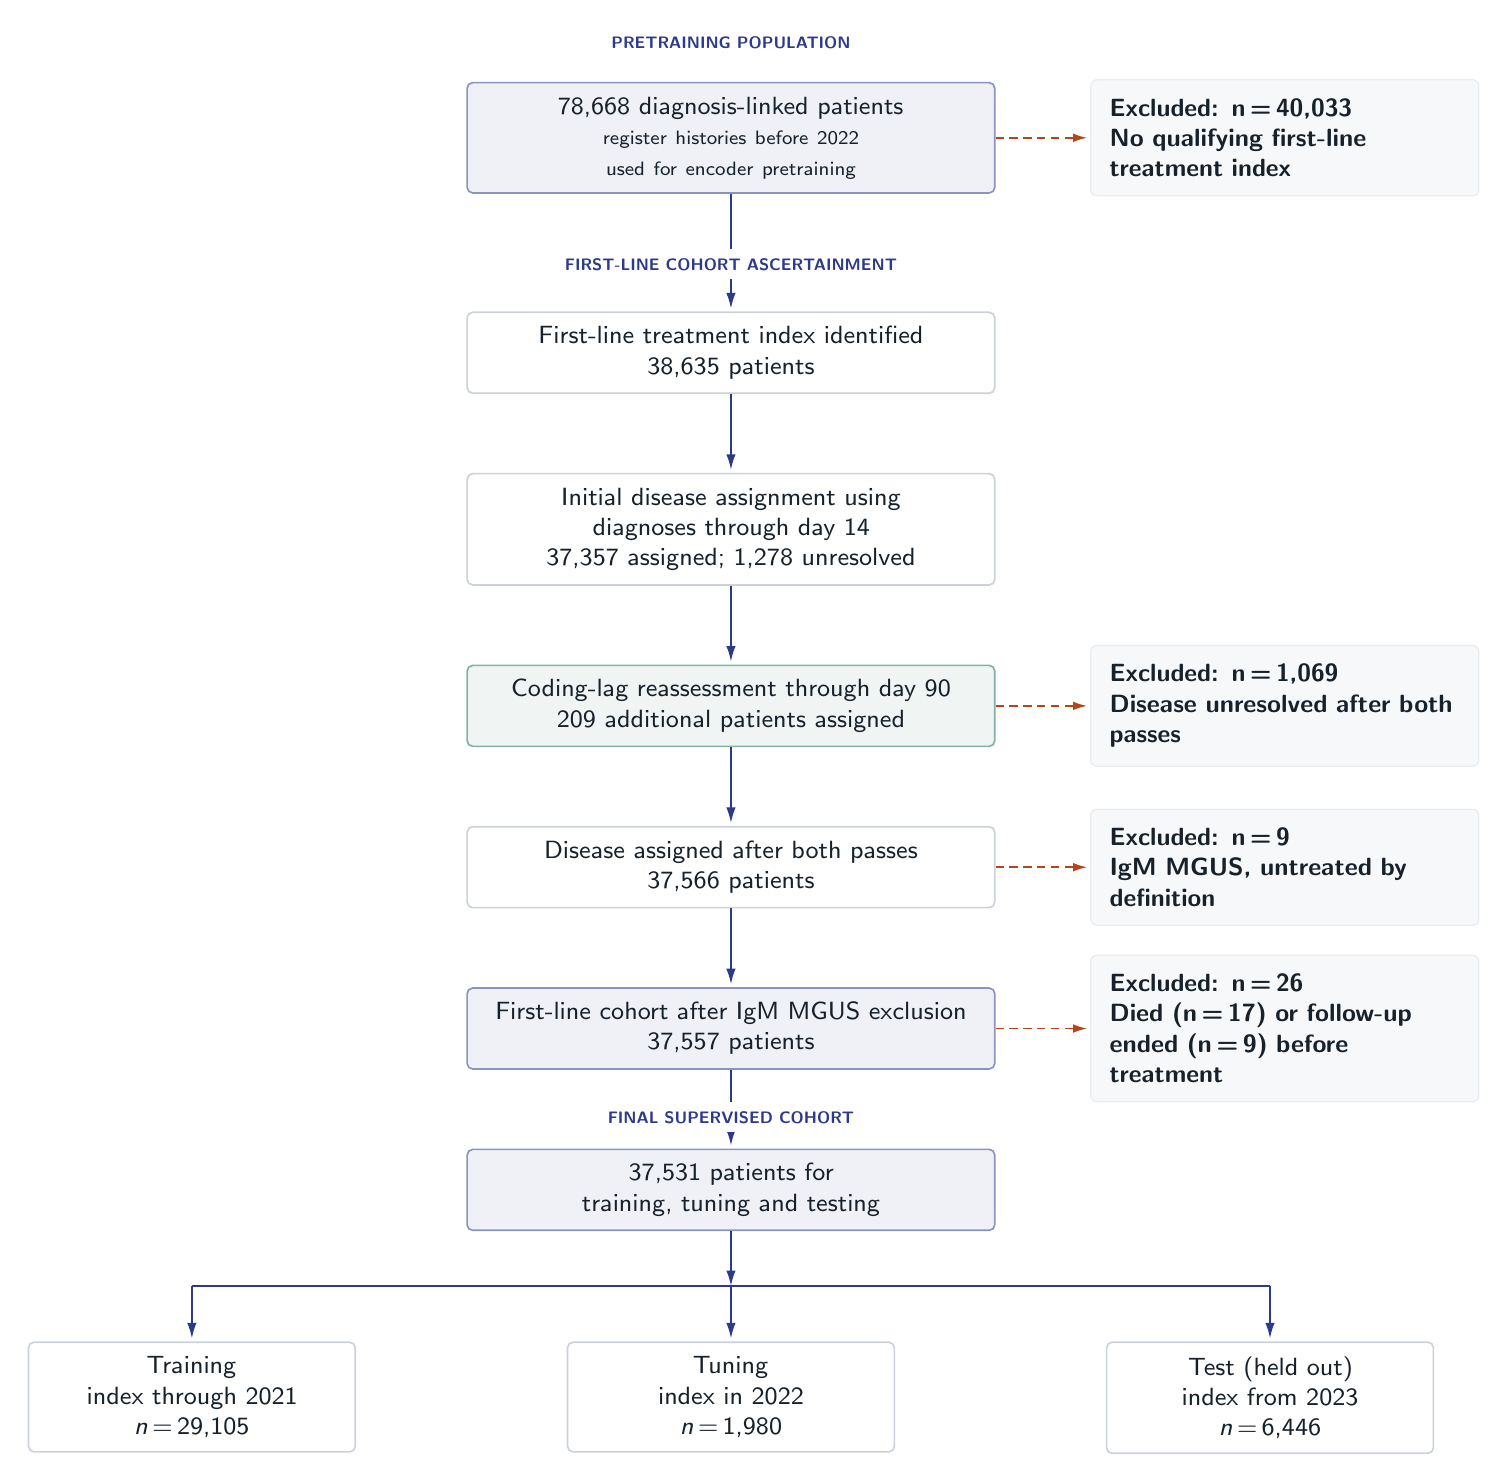
\begin{tikzpicture}[opera,node distance=10mm and 12mm,
    every node/.append style={execute at begin node={\hyphenpenalty=10000\exhyphenpenalty=10000}}]
  \node[stageblue,text width=6.1cm] (pretrainbox)
    {78,668 diagnosis-linked patients\\{\scriptsize register histories before 2022 used for encoder pretraining}};
  \node[eyebrow,above=3mm of pretrainbox] (pretrainlabel) {PRETRAINING POPULATION};
  \node[eyebrow,below=7mm of pretrainbox] (branchlabel)
    {FIRST-LINE COHORT ASCERTAINMENT};
  \node[stage,text width=6.1cm,below=4mm of branchlabel] (index)
    {First-line treatment index identified\\38,635 patients};
  \node[stage,text width=6.1cm,below=of index] (pass1)
    {Initial disease assignment using diagnoses through day 14\\37,357 assigned; 1,278 unresolved};
  \node[stageteal,text width=6.1cm,below=of pass1] (pass2)
    {Coding-lag reassessment through day 90\\209 additional patients assigned};
  \node[stage,text width=6.1cm,below=of pass2] (classified)
    {Disease assigned after both passes\\37,566 patients};
  \node[stageblue,text width=6.1cm,below=of classified] (firstline)
    {First-line cohort after IgM MGUS exclusion\\37,557 patients};
  \node[stageblue,text width=6.1cm,below=of firstline] (supervised)
    {37,531 patients for training, tuning and testing};

  \foreach \a/\b in {index/pass1,pass1/pass2,
                       pass2/classified,classified/firstline,firstline/supervised}
    \draw[flowblue,shorten >=1pt] (\a.south) -- (\b.north);
  \draw[flowblue,shorten >=1pt] (pretrainbox.south) -- (index.north);
  \node[eyebrow,fill=white,inner xsep=2mm] at (branchlabel) {FIRST-LINE COHORT ASCERTAINMENT};
  \node[eyebrow,fill=white,inner xsep=2mm,above=2mm of supervised]
    {FINAL SUPERVISED COHORT};

  % Mutually distinct exits from the central first-line flow.
  \node[softpanel,text width=4.45cm,align=left,right=of pretrainbox] (noindex)
    {\bfseries Excluded: \textit{n}\,=\,40{,}033\\No qualifying first-line treatment index};
  \node[softpanel,text width=4.45cm,align=left,right=of pass2] (unresolved)
    {\bfseries Excluded: \textit{n}\,=\,1{,}069\\Disease unresolved after both passes};
  \node[softpanel,text width=4.45cm,align=left,right=of classified] (secondary)
    {\bfseries Excluded: \textit{n}\,=\,9\\IgM MGUS, untreated by definition};
  \node[softpanel,text width=4.45cm,align=left,right=of firstline] (nosurvival)
    {\bfseries Excluded: \textit{n}\,=\,26\\Died (\textit{n}\,=\,17) or follow-up ended (\textit{n}\,=\,9) before treatment};
  \draw[relation,draw=OperaSienna,shorten >=1pt] (pretrainbox.east) -- (noindex.west);
  \draw[relation,draw=OperaSienna,shorten >=1pt] (pass2.east) -- (unresolved.west);
  \draw[relation,draw=OperaSienna,shorten >=1pt] (classified.east) -- (secondary.west);
  \draw[relation,draw=OperaSienna,shorten >=1pt] (firstline.east) -- (nosurvival.west);

  \node[stage,text width=3.55cm,below left=14mm and 14mm of supervised] (train)
    {Training\\index through 2021\\\textit{n}\,=\,29{,}105};
  \node[stage,text width=3.55cm,below=14mm of supervised] (tune)
    {Tuning\\index in 2022\\\textit{n}\,=\,1{,}980};
  \node[stage,text width=3.55cm,below right=14mm and 14mm of supervised] (held)
    {Test (held out)\\index from 2023\\\textit{n}\,=\,6{,}446};
  \coordinate (split) at ($(supervised.south)+(0,-7mm)$);
  \draw[flowblue] (supervised.south) -- (split);
  \draw[draw=OperaIndigo,line width=0.75pt]
    (train.north |- split) -- (held.north |- split);
  \foreach \dest in {train,tune,held}
    \draw[flowblue,shorten >=1pt] (\dest.north |- split) -- (\dest.north);

\end{tikzpicture}
}
  \caption{\textbf{Study population.} Of 78,668 adults in DALY-CARE with a
  lymphoid cancer or related diagnosis, whose pre-2022 histories were used for
  pretraining, 37,557 started first-line treatment and 37,531 were assigned to
  the training (to 2021), tuning (2022) or test (from 2023) period. Subtypes
  were assigned from diagnoses up to 14 days after treatment start, with
  reassessment up to day 90 for late-coded diagnoses. Counts are unique patients. Outcome-specific risk sets and detailed attrition are given in the Supplementary Methods. \placeholder{Counts pending final reconciliation.}}
  \label{fig:cohort-flow}
\end{figure}

\section*{Supplementary Methods: model and analysis details}
% Detailed methods moved from the main Methods.
\subsection*{Sequence encoder and supervised training}
Our sequence models build on CORE-BEHRT \citep{odgaard2024core}, adapted to a
causal encoder with next-event pretraining and multi-outcome competing-risk
prediction. Each patient's history was represented as a chronological sequence
of diagnoses, procedures, medications, laboratory results (discretised into
value bins) and hospital contacts, preceded by sex and age. A causal transformer
encoder \citep{vaswani2017attention} with a hidden size of 256, four layers and
four attention heads, and a scaled Time2Vec encoding of time
\citep{kazemi2019time2vec}, was pretrained to predict the next event over a
context of 8,192 events. \placeholder{Number of individuals and events,
training budget and selected epoch.} This encoder initialised every supervised
model in the main comparisons.

\subsection*{Supervised training across diseases and outcomes}
Every supervised model consisted of the pretrained encoder, trained further,
and a linear head that produced, for each outcome, piecewise-constant hazards
for the outcome and for competing death, building on neural interval-hazard and
competing-risk models \citep{gensheimer2019nnetsurvival,lee2018deephit}.
Cumulative incidence at each horizon was derived from these hazards. The loss
was a binary cross-entropy at each horizon: patients with the event before the
horizon were positive, patients who died of another cause or were followed
beyond the horizon were negative, and patients censored earlier did not
contribute at that horizon. Losses were averaged within each outcome and then
across endpoints, where the grade variants of one laboratory finding (grade
$\geq$2 and $\geq$3) and nested definitions of the same finding formed one
endpoint (69 outcomes, 52 endpoints), so that a finding defined at two grades
did not count twice. This weighting is separate from the clinical domains used
to present results, which group related outcomes for display only.

The four supervision scopes differed only in which cells of the
disease-by-outcome grid---one outcome in one disease---provided labels
(\cref{fig:supervision-grid}); we use ``cell'' for such a combination
throughout. A specialist learned one outcome
in one disease; a disease-pooled model learned one outcome across all diseases;
an outcome-pooled model learned all outcomes within one disease; and the joint
model learned all outcomes in all diseases. Every model predicted all six
horizons and was trained for up to 30 epochs, stopping after five epochs
without improvement in tuning loss, with the same optimiser, batch size and
sampling settings, and every comparison used the same target patients, labels
and horizons. Because equal epochs do not mean equal optimisation steps or
computation, we report both for each scope.

\subsection*{Outcome panel}
We predicted 69 outcomes covering disease course (second-line treatment,
treatment failure, transformation, new malignancy and death), infection,
haematological toxicity and transfusion, kidney, liver and coagulation
toxicity, electrolyte and metabolic disturbances, cardiovascular events and
acute care, each at 30, 60, 90, 180, 365 and 730 days. Laboratory outcomes used
grading thresholds aligned with, but not identical to, the Common Terminology
Criteria for Adverse Events \citep{nci2025ctcae}, with baseline-aware thresholds
when pre-treatment values were already abnormal; infection was additionally
captured through antimicrobial treatment, which we label as such. A patient
contributed to an outcome only if it was ascertainable for them---for example,
if laboratory follow-up was available---and was otherwise treated as missing
rather than negative. Death was a competing event for every non-fatal outcome.
The 69 outcomes were selected from 87 candidates by a prespecified rule based on
training and tuning event counts at one year, without held-out data
(Supplementary Methods S8). Definitions, code lists and risk-set sizes are
given in Supplementary Methods S5--S9.

\subsection*{Tabular comparators: features and tuning}
For each disease--outcome cell and horizon, we trained gradient-boosted trees
(XGBoost; \citealp{chen2016xgboost}) and ridge-penalised logistic regression on the
same patients, labels and competing-event handling as the neural models. Their
features came from the pipeline of our earlier DLBCL study
\citep{werling2026dlbcl}: using timeseriesflattener
\citep{bernstorff2023tsflattener}, prescriptions, laboratory results,
procedures and referrals, pathology codes, diagnoses, blood cultures and
microbiology were summarised over 90-day, one-year and three-year windows before
the index date, with aggregates suited to each source (counts and distinct
counts for codes; latest, minimum, maximum, variance and slope for laboratory
values). Variables recorded for fewer than 10\% of training patients were
represented by per-source counts of such rare occurrences. To give the tabular
and sequence models the same information, quality-registry variables such as
stage and performance status were removed, and age and sex at the index date
were added. Unlike the earlier study, no LASSO preselection was applied.
Numeric features were median-imputed with missingness indicators and
standardised, and categorical features one-hot encoded, with all preprocessing
fitted on training data. Hyperparameters were chosen for each cell by log loss
on the tuning set from a prespecified grid: for XGBoost, shallow trees (depth
1--3), deeper trees (depth 4 and 6) and the setting of the earlier study
(depth 8, learning rate 0.01, up to 3,000 trees), with the number of trees also
chosen on the tuning set; for logistic regression, the penalty strength along
a seven-value path ($C$ from $3\times10^{-4}$ to 1, fitted with warm starts). Neither model was class-reweighted, so both produce
probabilities that can be compared directly. \placeholder{Confirm against the
delivered feature export: anchoring at first-line treatment, source list and
number of features.}

As a reference outside the information-matched comparison, XGBoost was also
trained for each cell with the clinical quality-registry variables recorded at
diagnosis added to the same features (performance status, stage, lactate
dehydrogenase, extranodal involvement, B symptoms and cytogenetic risk where the
registry for the disease records them; \placeholder{final list}). Values were
taken as recorded at diagnosis, left missing where not recorded, and handled by
the same missingness indicators; hyperparameters were tuned on the same grid.
The sequence models never saw these variables, so this arm estimates what the
curated registry adds, not a like-for-like comparison.

\subsection*{Comparison with clinical prognostic indices}
The quality registries record, for each patient, the prognostic index scored at
diagnosis (for example the IPI, FLIPI, MIPI, CLL-IPI or ISS) and its risk
category (low, intermediate or high), before treatment started. Every index
recorded for at least 50 patients of a subtype, and every index used in more
than one subtype pooled across all subtypes recording it, was compared with the joint
model's predicted two-year risk of treatment failure, with death part of the
endpoint, in the patients who had that index. For DLBCL we also computed the
NCCN-IPI from the components recorded in the lymphoma registry, following
the original definition \citep{zhou2014nccnipi}: age (41--60, 61--75 and
over 75 years: 1, 2 and 3 points), LDH relative to the upper limit of normal
(205~U/L, or 255~U/L from age 70; ratio above 1 and above 3: 1 and 2 points),
Ann Arbor stage III--IV (1 point), involvement of bone marrow, central nervous
system, liver, gastrointestinal tract or lung (1 point), and performance
status $\geq$2 (1 point); low 0--1, low-intermediate 2--3, high-intermediate
4--5, high $\geq$6. Patients missing any component were not scored.

Model risk groups were fixed on tuning patients with known two-year status and
applied unchanged to the test set. The low cutoff was the highest predicted
risk at which the group below it, of at least 20 patients, had an observed risk
no higher than the index's low-risk category. The high cutoff was the predicted
risk at which the model's specificity equalled that of the index's high-risk
category, so that both flagged the same proportion of patients without the
event; this is also the operating point marked in the precision--recall
comparison. Patients between the two cutoffs were divided in the proportions
of the index's intermediate categories (one for the registry indices, two for
the NCCN-IPI). Anchoring both ends to the index makes the groups directly
comparable while leaving the model free to differ: a model that ranks patients
better places more patients at low risk at the same risk, and captures more
events at the same specificity. For each index and each system we report group
size, observed risk, and the sensitivity and specificity of classifying a
patient in that group or higher, and, for the model, the observed risk in its
highest-risk 5\% and 10\% of patients, which the index cannot resolve within
its top category. As a sensitivity analysis, model groups were instead given
exactly the index's group sizes. Discrimination used the index category (or
NCCN-IPI points) as an ordinal score.

\subsection*{Routing formulation and selection}
To test whether a joint model benefits from conditioning its predictions on
disease and outcome beyond ordinary shared learning, we compared the joint
model with a routed model trained on the same panel. In the routed model, the
patient representation
$h_i$ is adjusted for each target outcome $k$ by a weighted combination of
small residual adapters, one per disease and one per outcome:
\begin{equation}
 \begin{aligned}
 h_{ik}&=h_i+\lambda\sum_s\pi_{iks}\,c_s\,A_s(h_i),\\
 A_s(h)&=U_s\,\mathrm{GELU}(V_s h),
 \qquad c_s=\frac{e_s}{e_s+\tau}.
 \end{aligned}
 \label{eq:router}
\end{equation}
where $A_s$ is a low-rank adapter for source $s$, the weights $\pi_{iks}$ are
computed from the patient, the patient's disease and the target outcome, and
$c_s$ shrinks the contribution of sources with few training events $e_s$. The
adapted representation enters the same linear head as in the joint model. Each adapter was
updated only by the supervision of its own disease or outcome. The approach
relates to mixtures of experts and parameter-efficient adapters
\citep{jacobs1991adaptive,ma2018mmoe,houlsby2019adapters,pfeiffer2021adapterfusion}.

The router configuration was chosen on the tuning set in a short prespecified
sequence: which adapter banks to include (none, disease, outcome or both), then
the adapter rank, then the form of the routing query. A simpler configuration
was preferred unless a more complex one improved tuning performance beyond a
prespecified margin, and a routed model with no adapters was required to
match the joint model before differences between adapter banks were interpreted.
\placeholder{Insert the selected configuration.} Because a target outcome
already has its own prediction head, an outcome adapter bank must add value
beyond that head; route weights describe how the model allocates corrections
and are not interpreted as evidence of relationships between diseases.



\begin{figure}[!htbp]
  \centering
  \resizebox{0.96\textwidth}{!}{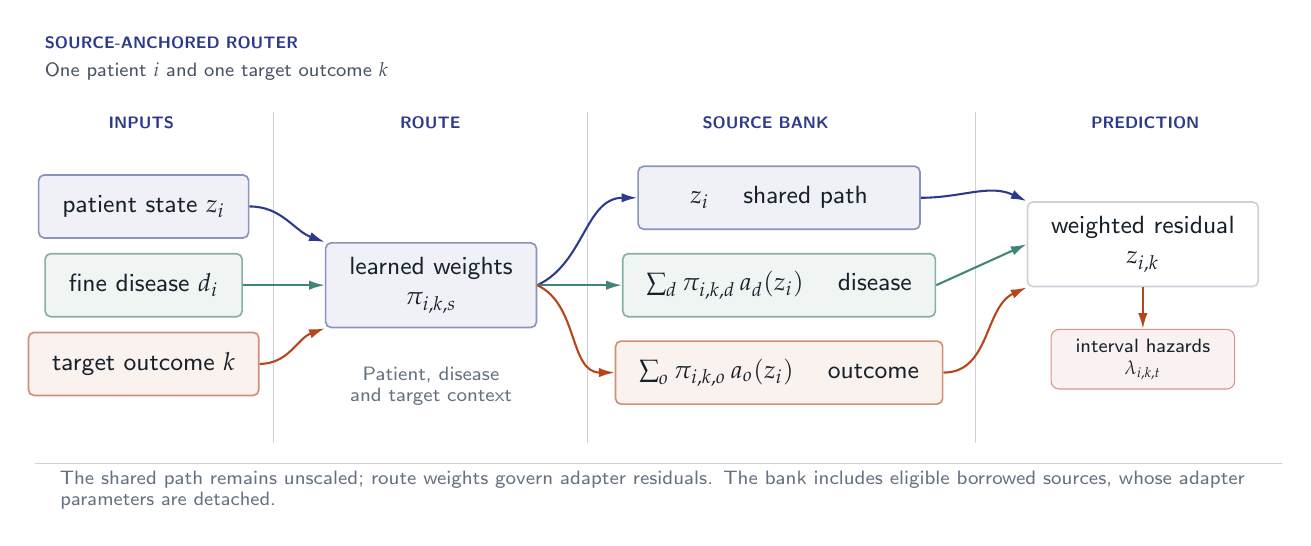
\begin{tikzpicture}[opera,x=1cm,y=1cm]
  % One target prediction, represented as four clearly separated stages.
  \node[eyebrow,anchor=west] at (0,0) {SOURCE-ANCHORED ROUTER};
  \node[labelsmall,anchor=west] at (0,-.36)
    {One patient $i$ and one target outcome $k$};

  \node[eyebrow] at (1.35,-1.02) {INPUTS};
  \node[eyebrow] at (5.02,-1.02) {ROUTE};
  \node[eyebrow] at (9.28,-1.02) {SOURCE BANK};
  \node[eyebrow] at (14.10,-1.02) {PREDICTION};
  \draw[divider] (3.03,-.88)--(3.03,-5.08);
  \draw[divider] (7.02,-.88)--(7.02,-5.08);
  \draw[divider] (11.94,-.88)--(11.94,-5.08);

  % Input identities are not source representations: the encoder supplies z.
  \node[stageblue,minimum width=2.18cm] (patient) at (1.38,-2.08)
    {patient state $z_i$};
  \node[stageteal,minimum width=2.18cm] (disease) at (1.38,-3.08)
    {fine disease $d_i$};
  \node[stagewarm,minimum width=2.18cm] (target) at (1.38,-4.08)
    {target outcome $k$};

  \node[stageblue,minimum width=2.48cm,minimum height=1.04cm]
    (router) at (5.03,-3.08) {learned weights\\$\pi_{i,k,s}$};
  \draw[flowblue] (patient.east) to[out=0,in=160] (router.north west);
  \draw[flowteal] (disease.east)--(router.west);
  \draw[flowwarm] (target.east) to[out=0,in=200] (router.south west);
  \node[captionnote,text width=3.40cm] at (5.03,-4.36)
    {Patient, disease and target context};

  % The three rows are categories, not a claim that only three sources exist.
  \node[stageblue,minimum width=3.58cm] (shared) at (9.45,-1.97)
    {$z_i$ \quad shared path};
  \node[stageteal,minimum width=3.58cm] (dsrc) at (9.45,-3.08)
    {$\sum_d\pi_{i,k,d}\,a_d(z_i)$ \quad disease};
  \node[stagewarm,minimum width=3.58cm] (osrc) at (9.45,-4.19)
    {$\sum_o\pi_{i,k,o}\,a_o(z_i)$ \quad outcome};
  \draw[flowblue] (router.east) to[out=25,in=180] (shared.west);
  \draw[flowteal] (router.east)--(dsrc.west);
  \draw[flowwarm] (router.east) to[out=-25,in=180] (osrc.west);

  \node[stage,minimum width=2.33cm] (mix) at (14.07,-2.56)
    {weighted residual\\$z_{i,k}$};
  \node[outcome,minimum width=2.33cm] (hazards) at (14.07,-4.02)
    {interval hazards\\$\lambda_{i,k,t}$};
  \draw[flowblue] (shared.east) to[out=0,in=155] (mix.north west);
  \draw[flowteal] (dsrc.east)--(mix.west);
  \draw[flowwarm] (osrc.east) to[out=0,in=205] (mix.south west);
  \draw[flowwarm] (mix.south)--(hazards.north);

  \draw[divider] (0,-5.34)--(15.84,-5.34);
  \node[captionnote,anchor=west,text width=15.40cm,align=left]
    at (.20,-5.68)
    {The shared path remains unscaled; route weights govern adapter residuals. The bank includes eligible borrowed sources, whose adapter parameters are detached.};
\end{tikzpicture}
}
  \caption{\textbf{Source-anchored disease--outcome routing.} For each patient
  and target outcome, the router mixes a shared representation with residual
  adapters indexed by fine disease and outcome. Its weights depend on the
  patient, disease and target; sources with no training support are masked and
  low-event sources are shrunk. An adapter is updated by its own eligible
  supervision, while borrowed adapter parameters are detached. The mixed
  representation enters a shared linear head for interval hazards and
  cumulative incidence. This is a model schematic, not an empirical route-weight
  or performance plot.}
  \label{fig:source-router}
\end{figure}


\subsection*{Hierarchy for effect heterogeneity}
The primary evidence is the paired effect in each disease--outcome cell with
its patient-bootstrap interval. Many cells are small, so their raw estimates
are noisy and rankings of individual cells are unreliable. We therefore also
fit a deliberately simple Bayesian hierarchical model whose purpose is partial
pooling: each cell's effect is the panel mean plus a disease effect, an outcome
effect and a cell-specific deviation, so that a noisy cell is shrunk towards
what similar cells show, by an amount the data determine. The model answers
two questions: how large is the typical effect, and how much does it vary
between diseases and between outcomes? The cell estimates are not treated as
independent: their sampling covariance, taken from the shared patient-bootstrap
draws, enters the likelihood, because the same patients contribute to every
outcome within a disease.

Whether effects depend on the amount of training data available for the
target is a separate question; we do not assume a linear relationship.
A low-dimensional spline still constrains smoothness and complexity. The cell effect is allowed to vary smoothly with log training
events through a cubic spline with few knots and a shrinkage prior, to regularise departures from a flat relationship; the prior still affects
the fitted shape and is assessed in sensitivity checks. As a transparent check
that does not depend on smoothing, cells are also grouped into prespecified
bins of training events (fixed before held-out evaluation) and the mean effect
is estimated within each bin. Within each
question, the model fits the independent effects directly (for pooling:
disease pooling, outcome pooling and their interaction); conditional and
combined contrasts are exact sums of these, so all reported pooling contrasts
are mutually consistent. Priors
are weakly informative on each metric's scale and checked with prior
predictive simulation; convergence and posterior predictive checks are
reported. Posterior probabilities of benefit, harm and practical equivalence
use a prespecified tolerance. Raw paired estimates are always shown alongside.
\placeholder{Insert locked priors, tolerances, support-bin edges and sampling
diagnostics.}


\FloatBarrier

\clearpage
\section*{Supplementary Methods: evaluation and reporting}
% Evaluation methods in reported form; empirical tables are filled from the locked analysis.
\subsection*{Risk sets and paired comparisons}
The unit of evaluation was one disease--outcome--horizon combination. Its risk
set was determined by eligibility and ascertainment of the outcome, not by the
models compared. For each split we report eligible patients, outcome events,
competing deaths and patients whose status was unknown at the horizon. Each
paired comparison used the patients with predictions from both models, so
different contrasts may rest on different risk sets, and their denominators are reported. Cells in which a model could not be fitted or a metric could not be
estimated remain in the coverage inventory with the reason
(\cref{fig:supp-coverage}) and are not treated as zero effects.

Superiority among evaluable cells was kept separate from coverage of
additional cells. A pooled model could predict cells in which no specialist
could be fitted. These cells have absolute performance estimates but no paired
specialist comparison, and were not imputed into pooled averages. Outcome
definitions and the reconstruction of treatment lines are in the appended
data-definition supplement.

\subsection*{Clinical prognostic indices}
Each index was evaluated in the population and for the endpoint closest to
those it was developed for, at the same prediction time. Original and evaluated
endpoints and horizons are listed side by side, and a shorter available
horizon is not presented as a reproduction of a longer development horizon.
All methods in an index comparison used the same patients, those with the index
recorded at diagnosis, and how often it was recorded is reported by disease and
calendar period. Index categories were used as recorded. Because the sequence
and tabular models read the wider history, a gain over an index is a gain of
the whole pipeline and does not separate the model from the information it
receives.

Index categories are not individual probabilities. They were used for ranking
and stratification. Brier scores and calibration of an index would require a
probability mapping fitted on development data, which we did not use.
\placeholder{Index, version, population and availability inventory from the
secure analysis.}

\subsection*{Risk groups, age and operating points}
Continuous model risks were converted to groups fixed at baseline with cutoffs
selected on tuning data, while index groups kept their original definitions.
Kaplan--Meier estimates describe endpoints that include death, and
Aalen--Johansen estimates non-fatal endpoints with death as a competing event.
Group sizes, events and 95\% bootstrap intervals accompany every estimate.
Patients without a recorded index were not included in index comparisons.

In the age figures, patient counts, mean predicted risk and observed risk are
shown as separate rows on the same age bands and groups. The predicted row is
the sequence model's mean probability, also within index categories. The index itself supplies no probability. Estimates are suppressed for cells with fewer
than ten patients, while counts remain visible.

Operating points used thresholds fixed on tuning data, so the specificity
matched on tuning data is not exactly matched in the test period. We report
the achieved sensitivity, specificity, positive and negative predictive values
and patient counts. Confusion counts use patients with known status at the
horizon, and the number excluded by censoring is reported. Censoring-weighted quantities are labelled as such.

For the panel as a whole, every model was also evaluated at six decision
points, each fixed per model, cell and horizon on that model's tuning
predictions. The first flagged as many tuning patients as had the event, so
that every model raised the same number of alerts. The second and third
maximised Youden's index and the MCC. The remaining three were the lowest
thresholds with a tuning specificity of at least 80\%, 90\% and 95\%. The test
period then shows how far the achieved specificity drifts from its tuning
target. For each decision point we report the threshold, the confusion matrix,
sensitivity, specificity, positive and negative predictive values, MCC and the
share of patients flagged, with 95\% intervals from the shared patient
bootstrap and paired differences between the joint model and XGBoost, the
joint model and the specialist, and the routed and joint models. Confusion
counts below five are suppressed in exported tables, as required by the secure
environment. Cells with fewer than five tuning events or non-events have no
decision point.

\subsection*{Censoring, calibration and robustness}
Censoring-weighted and known-status estimates answer different questions and
are reported separately, and the known-status analysis is a prespecified
sensitivity analysis. For the censoring weights we report the censoring model,
the censoring survival at each horizon and the distribution of weights. Long
horizons with little follow-up are flagged where estimates are unstable.

Calibration is reported as calibration-in-the-large, the calibration slope
where estimable, and reliability curves for outcomes chosen by a fixed rule. No
model was recalibrated on test data. Sensitivity analyses by horizon, calendar
year, amount of recorded history and timing of the subtype diagnosis are
reported on their own risk sets. Raw paired effects are reported with the
hierarchical summaries, and the support curve, unsmoothed and binned analyses
are treated as views of the same data rather than independent replications.

\subsection*{Patient representations}
The representation figures show the same test patients at five stages: local
pretraining, the locally pretrained joint model, national pretraining, national
pretraining with local adaptation, and the nationally initialised joint model.
For each stage, the projection was fitted on tuning patients and applied
unchanged to test patients, so coordinates are comparable within a stage but
not between stages. For every stage we record the checkpoint, the layer and
pooling used, the input cutoff and truncation. Clusters and changes in
separation are descriptive. They do not show differences in prediction,
biological mechanisms or the effect of transfer. Only kernel-smoothed
summaries over at least \placeholder{N} patients are shown, following the
disclosure rules of the secure environment.

\subsection*{Numerical tables}
The supplementary tables give, for every cell, the risk sets, absolute
performance, paired effects, index comparisons, calibration, operating points
and sensitivity analyses, together with training resources. Each model was
trained once, so intervals describe sampling of test patients only. Readable
summaries accompany the complete cell-level files.
\placeholder{Populate from the locked analysis.}

\IfFileExists{tables/generated/supplement_tables.tex}{%
  \subsection*{Reviewed numerical summaries}
  \input{tables/generated/supplement_tables}
}{%
  \noindent\placeholder{Reviewed aggregate summary tables have not yet been
  exported. Complete cell-level numerical tables will accompany the figures.}
}

\clearpage
\section*{Supplementary figures}

\begin{figure}[H]
  \resultfigure[\textwidth]{supp_routing}{Routing}{Routed versus joint
    and adapter-bank comparison.}
  \caption{\textbf{Routed versus joint model, and adapter-bank comparisons.}
  \textbf{A}, Paired
  one-year AUC gain of the routed over the joint model by clinical domain, with the prespecified margin of practical equivalence shaded. \textbf{B},
  Panel gains of adapter banks trained under the same protocol: no adapters
  versus the joint model (a check that the architecture alone changes nothing),
  disease adapters, outcome adapters, each given the other, both, and their
  interaction. The router configuration was chosen on the tuning set.}
  \label{fig:routing}
\end{figure}

\begin{figure}[p]
  \resultfigure[\textwidth]{supp_strategy}{Joint model versus per-cell
    selection}{Joint model against the specialist and the tuning-selected best model.}
  \caption{\textbf{Joint model versus the best model selected for each cell.}
  \textbf{A}, Test AUC of the joint model against the specialist in each cell, with point size reflecting training events. \textbf{B}, Against the best of
  the specialist, disease-pooled and outcome-pooled models chosen per cell on
  the tuning set. \textbf{C}, Which model was chosen, by clinical domain.}
  \label{fig:strategy}
\end{figure}


\begin{figure}[p]
  \centering
  \resizebox{\textwidth}{!}{% Supervision scopes drawn as four copies of the Fig. 2B disease-outcome matrix:
% same axes, rows/columns, ellipses, cell geometry, lavender gradient, sienna
% target and teal borrowing spokes. Filled cells are supervised tasks; pale
% outlined cells are present in the panel but not supervised by that fit.
% Lines are illustrative sharing paths, not learned gates or measured routes.
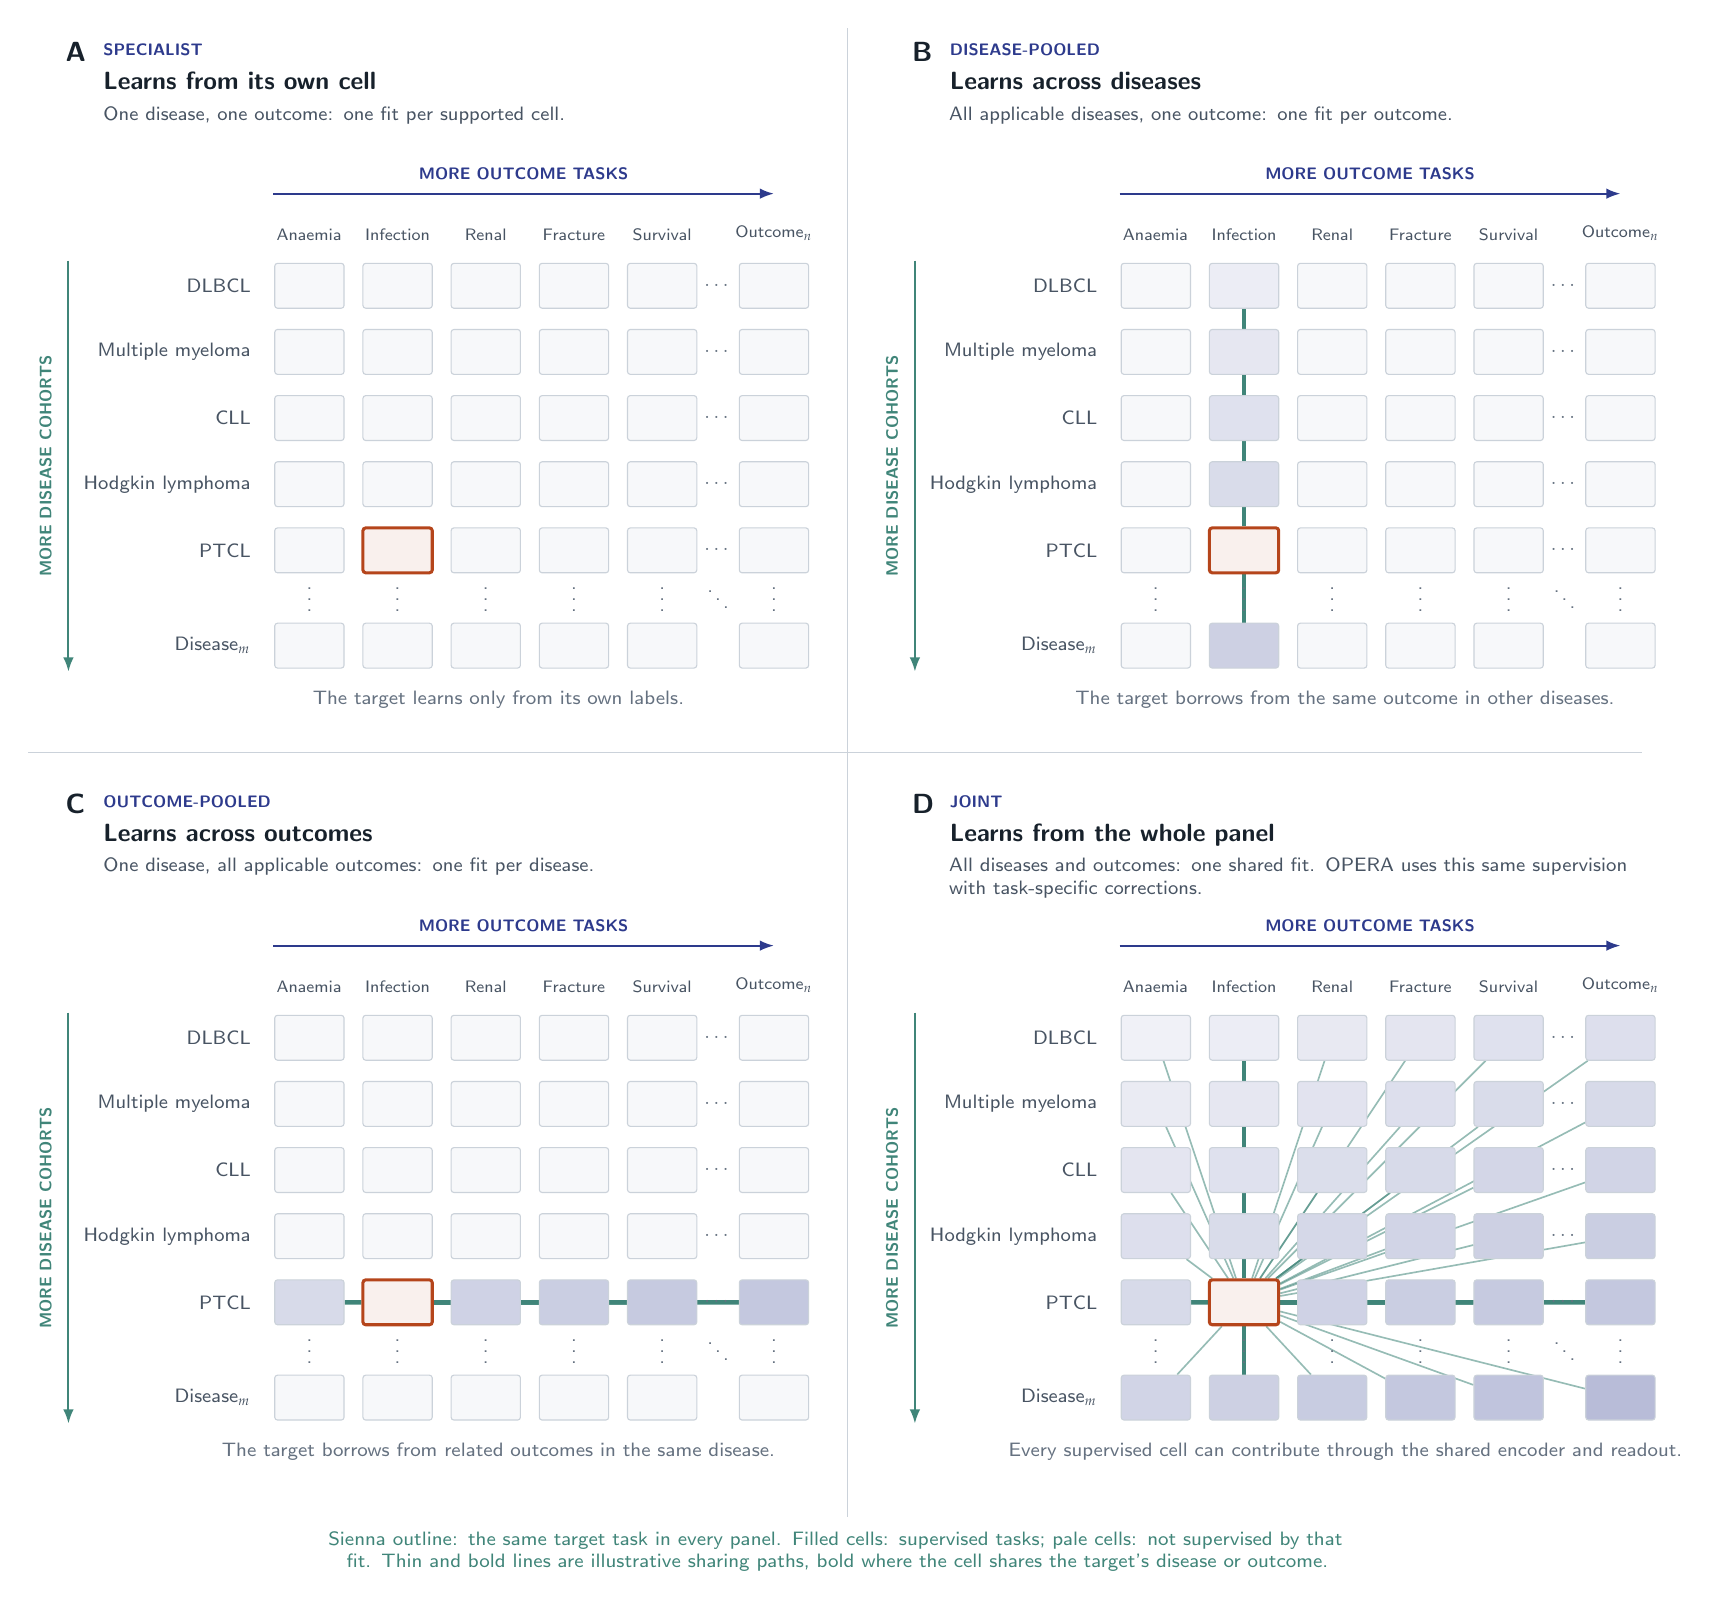
\begin{tikzpicture}[opera,x=1cm,y=1cm]
\foreach \scopeid/\sx/\sy/\letter/\eyebrowtext/\title/\sub/\note in {
 S/0/0/A/{SPECIALIST}/{Learns from its own cell}/{One disease, one outcome: one fit per supported cell.}/{The target learns only from its own labels.},
 D/10.75/0/B/{DISEASE-POOLED}/{Learns across diseases}/{All applicable diseases, one outcome: one fit per outcome.}/{The target borrows from the same outcome in other diseases.},
 O/0/-9.55/C/{OUTCOME-POOLED}/{Learns across outcomes}/{One disease, all applicable outcomes: one fit per disease.}/{The target borrows from related outcomes in the same disease.},
 J/10.75/-9.55/D/{JOINT}/{Learns from the whole panel}/{All diseases and outcomes: one shared fit. OPERA uses this same supervision with task-specific corrections.}/{Every supervised cell can contribute through the shared encoder and readout.}}{
\begin{scope}[xshift=\sx cm,yshift=\sy cm]
 \node[panelletter,anchor=north west] at (0,0) {\letter};
 \node[eyebrow,anchor=north west] at (.48,-.03) {\eyebrowtext};
 \node[heading,anchor=north west] at (.48,-.38) {\title};
 \node[labelsmall,anchor=north west,align=left,text width=8.6cm] at (.48,-.82) {\sub};
 \begin{scope}[yshift=-5mm]
 % Axes exactly as in Fig. 2B.
 \draw[-{Latex[length=1.8mm]},draw=OperaIndigo,line width=.75pt] (2.76,-1.55)--(9.12,-1.55);
 \node[eyebrow,text=OperaIndigo] at (5.94,-1.30) {MORE OUTCOME TASKS};
 \foreach \r/\disease in {0/DLBCL,1/Multiple myeloma,2/CLL,3/Hodgkin lymphoma,4/PTCL}
  \node[labelsmall,anchor=east] at (2.60,-2.72-.84*\r) {\disease};
 \draw[-{Latex[length=1.8mm]},draw=OperaTeal,line width=.75pt] (.16,-2.40)--(.16,-7.62);
 \node[eyebrow,text=OperaTeal,rotate=90] at (-.13,-5.01) {MORE DISEASE COHORTS};
 \foreach \col/\outcome in {0/Anaemia,1/Infection,2/Renal,3/Fracture,4/Survival}
  \node[font=\sffamily\fontsize{6.2}{7}\selectfont,text=OperaInkSecondary,
   align=center,text width=1.05cm,anchor=south] at (3.22+1.12*\col,-2.27) {\outcome};
 \node[font=\sffamily\fontsize{6.2}{7}\selectfont,text=OperaInkSecondary,
  align=center,text width=1.05cm,anchor=south] at (9.12,-2.27) {Outcome$_n$};
 % Main 5 x 5 block. Supervision depends on the scope; the target is row 4, column 1.
 \foreach \r in {0,...,4}{\foreach \col in {0,...,4}{
  \def\active{0}
  \if\scopeid D \ifnum\col=1 \def\active{1}\fi\fi
  \if\scopeid O \ifnum\r=4 \def\active{1}\fi\fi
  \if\scopeid J \def\active{1}\fi
  \def\tone{OperaPaper}
  \ifnum\active=1 \pgfmathtruncatemacro{\shade}{7+3*\r+2*\col}\edef\tone{OperaIndigo!\shade}\fi
  \node[rounded corners=.35mm,draw=OperaBorder,fill=\tone,
   minimum width=8.8mm,minimum height=5.7mm] (\scopeid m\r\col) at (3.22+1.12*\col,-2.72-.84*\r) {};
 }}
 \foreach \r in {0,...,4}{
  \node[font=\sffamily\scriptsize,text=OperaInkMuted] at (8.41,-2.72-.84*\r) {$\cdots$};
  \def\active{0}
  \if\scopeid O \ifnum\r=4 \def\active{1}\fi\fi
  \if\scopeid J \def\active{1}\fi
  \def\tone{OperaPaper}
  \ifnum\active=1 \pgfmathtruncatemacro{\shade}{16+3*\r}\edef\tone{OperaIndigo!\shade}\fi
  \node[rounded corners=.35mm,draw=OperaBorder,fill=\tone,
   minimum width=8.8mm,minimum height=5.7mm] (\scopeid n\r) at (9.12,-2.72-.84*\r) {};
 }
 \foreach \x in {3.22,4.34,5.46,6.58,7.70,9.12}{
  \node[font=\sffamily\scriptsize,text=OperaInkMuted] at (\x,-6.60) {$\vdots$};
 }
 \node[font=\sffamily\scriptsize,text=OperaInkMuted] at (8.41,-6.60) {$\ddots$};
 \node[labelsmall,anchor=east] at (2.60,-7.29) {Disease$_m$};
 \foreach \col in {0,...,4}{
  \def\active{0}
  \if\scopeid D \ifnum\col=1 \def\active{1}\fi\fi
  \if\scopeid J \def\active{1}\fi
  \def\tone{OperaPaper}
  \ifnum\active=1 \pgfmathtruncatemacro{\shade}{22+2*\col}\edef\tone{OperaIndigo!\shade}\fi
  \node[rounded corners=.35mm,draw=OperaBorder,fill=\tone,
   minimum width=8.8mm,minimum height=5.7mm] (\scopeid z\col) at (3.22+1.12*\col,-7.29) {};
 }
 \def\tone{OperaPaper}
 \if\scopeid J \def\tone{OperaIndigo!34}\fi
 \node[rounded corners=.35mm,draw=OperaBorder,fill=\tone,
  minimum width=8.8mm,minimum height=5.7mm] (\scopeid zn) at (9.12,-7.29) {};
 \node[rounded corners=.35mm,draw=OperaSienna,line width=1.1pt,fill=OperaSienna!8,
  minimum width=8.8mm,minimum height=5.7mm] (\scopeid target) at (4.34,-6.08) {};
 % Spokes from supervised cells only: bold when the cell shares the target's
 % outcome (column 1) or disease (row 4), thin otherwise, as in Fig. 2B.
 \begin{scope}[on background layer]
  \foreach \r in {0,...,4}{\foreach \col in {0,...,4}{
   \def\link{0}
   \if\scopeid D \ifnum\col=1 \def\link{1}\fi\fi
   \if\scopeid O \ifnum\r=4 \def\link{1}\fi\fi
   \if\scopeid J \def\link{1}\fi
   \ifnum\r=4 \ifnum\col=1 \def\link{0}\fi\fi
   \ifnum\link=1
    \def\bold{0}
    \ifnum\col=1 \def\bold{1}\fi
    \ifnum\r=4 \def\bold{1}\fi
    \ifnum\bold=1
     \draw[draw=OperaTeal,opacity=1,line width=1.6pt] (\scopeid m\r\col)--(\scopeid target);
    \else
     \draw[draw=OperaTeal,opacity=.55,line width=.6pt] (\scopeid m\r\col)--(\scopeid target);
    \fi
   \fi
  }}
  \if\scopeid O \draw[draw=OperaTeal,opacity=1,line width=1.6pt] (\scopeid n4)--(\scopeid target);\fi
  \if\scopeid D \draw[draw=OperaTeal,opacity=1,line width=1.6pt] (\scopeid z1)--(\scopeid target);\fi
  \if\scopeid J
   \foreach \r in {0,...,3}{\draw[draw=OperaTeal,opacity=.55,line width=.6pt] (\scopeid n\r)--(\scopeid target);}
   \draw[draw=OperaTeal,opacity=1,line width=1.6pt] (\scopeid n4)--(\scopeid target);
   \foreach \col in {0,2,3,4}{\draw[draw=OperaTeal,opacity=.55,line width=.6pt] (\scopeid z\col)--(\scopeid target);}
   \draw[draw=OperaTeal,opacity=1,line width=1.6pt] (\scopeid z1)--(\scopeid target);
   \draw[draw=OperaTeal,opacity=.55,line width=.6pt] (\scopeid zn)--(\scopeid target);
  \fi
 \end{scope}
 \node[captionnote,text width=8.5cm] at (5.60,-7.98) {\note};
 \end{scope}
\end{scope}
}
\draw[divider] (10.05,.05)--(10.05,-18.85);
\draw[divider] (-.35,-9.15)--(20.15,-9.15);
\node[labelsmall,text=OperaTeal,align=center,text width=18cm] at (9.90,-19.30)
 {Sienna outline: the same target task in every panel. Filled cells: supervised tasks; pale cells: not supervised by that fit.
 Thin and bold lines are illustrative sharing paths, bold where the cell shares the target's disease or outcome.};
\end{tikzpicture}
}
  \caption{\textbf{Supervision scopes on the disease--outcome matrix.} The matrix of \cref{fig:paradigms}E, with one target task
  (outlined) evaluated identically in every panel. Diseases are rows and
  outcomes are columns. \textbf{A}, A specialist learns one outcome in one disease. \textbf{B}, A disease-pooled model learns one outcome across all diseases. \textbf{C}, An outcome-pooled model learns all outcomes within one disease. \textbf{D}, The joint model learns all outcomes in all diseases.
  Filled cells indicate supervision, not performance. The routed model uses
  the same panel as the joint model and changes only how predictions are read
  out. Every model predicts all six horizons.}
  \label{fig:supervision-grid}
\end{figure}



\begin{figure}[p]
  \resultfigure{supp_clinical_score_age}{Risk groups by age}{Patient counts, predictions and observed risk separately.}
  \caption{\textbf{Model and IPI risk groups by age in DLBCL.} Patients with DLBCL and a
  recorded IPI, grouped by model risk group (left) and IPI category (right).
  Rows show, by age band, the number of patients, the mean predicted two-year
  treatment-failure-free survival and the observed Kaplan--Meier estimate, each
  with its 95\% bootstrap interval. Estimates are suppressed for cells with fewer than ten patients, but counts remain visible.}
  \label{fig:clinical-score-age}
\end{figure}

\begin{figure}[p]
  \resultfigure[0.95\textwidth]{supp_score_overview}{Comparison with each recorded prognostic index}
    {Survival by model risk group and by index category for each index and
    population.}
  \caption{\textbf{Model risk groups compared with each recorded prognostic
  index.} One row
  per index and the population it applies to, on patients with that index
  recorded at diagnosis. Left, survival (or freedom from the endpoint) by model risk group. Middle, the same by index category, on the same patients. Right, estimates at two years with 95\% CI (M, model, and I, index). Shaded bands are 95\%
  bootstrap intervals and the dashed line marks two years. Model cutoffs were
  fixed on tuning data for each index, matching its low-risk observed risk and
  high-risk specificity. Every index recorded for at least 50 patients of a
  subtype is shown, and the NCCN-IPI in DLBCL. Group sizes, observed risk,
  sensitivity and specificity of both systems are in Supplementary
  Table~\placeholder{S}. \placeholder{Endpoint per index.}}
  \label{fig:score-overview}
\end{figure}

\begin{figure}[p]
  \resultfigure{fig_clinical_score}{Operating points relative to the IPI}
    {A: precision--recall with matched-specificity operating point. B: model
    risk within index groups. C--D: incidence by age and risk group.}
  \caption{\textbf{Operating points and reclassification relative to the IPI
  in DLBCL.} \textbf{A},
  Precision--recall curves for treatment failure within two years (patients
  with known status at two years) for the model and for each IPI category
  threshold. The square marks the IPI high-risk category. Dotted lines project it onto the model's curve: straight up gives the model's precision at the IPI's recall, and straight right its recall at the IPI's precision. The diamond marks the model at a threshold chosen on tuning data to match the IPI's specificity. AP, average
  precision. \textbf{B}, Predicted two-year risk of each patient within each
  IPI category, coloured by whether treatment failed, with the model risk groups shaded. \textbf{C--D}, Two-year treatment-failure-free survival (95\% bootstrap
  interval) by age band and risk group for the model (\textbf{C}) and the IPI
  (\textbf{D}).}
  \label{fig:clinical-score}
\end{figure}

% One plate like the figure above for every recorded index, written by the
% clinical-scores step; copy its clinical_scores/ folder into the figure directory.
\IfFileExists{\resultfiguredir clinical_scores/supplement_clinical_scores.tex}{%
  \input{\resultfiguredir clinical_scores/supplement_clinical_scores.tex}}{}

\begin{figure}[p]
  \resultfigure[0.6\textwidth]{fig_who_benefits}{Gain by patient subgroup}
    {Paired Brier improvement of the joint model over the specialist and over
    XGBoost by patient subgroup.}
  \caption{\textbf{Gain from joint learning by patient subgroup.} Patient-weighted
  improvement in one-year Brier score ($\times$100, 95\% bootstrap CI) of the
  joint model over the specialist and over XGBoost, pooled across cells, by
  subgroups defined at the start of treatment. Positive values favour the
  joint model.}
  \label{fig:who-benefits}
\end{figure}

\begin{figure}[p]
  \resultfigure[0.9\textwidth]{supp_coverage}{Estimability}{Estimability of each
    disease--outcome cell.}
  \caption{\textbf{Estimability of disease--outcome cells.} Status of every
  disease--outcome cell at one year: all models evaluated, too few training
  events to train a specialist, no events in the test period, fit failed, or
  not applicable (sex- or disease-specific outcomes). Counts in the legend.}
  \label{fig:supp-coverage}
\end{figure}

\begin{figure}[p]
  \resultfigure[0.9\textwidth]{supp_support}{Training support}{Training
    events per cell and their cumulative distribution.}
  \caption{\textbf{Training events per disease--outcome cell.}
  \textbf{A}, Training events by one year in each disease--outcome cell (log scale, grey for none). \textbf{B}, Cumulative distribution across cells, with
  the support-bin edges used in the analysis marked.}
  \label{fig:supp-support}
\end{figure}

\begin{figure}[p]
  \resultfigure[0.9\textwidth]{supp_pooling_cells}{Cell-level pooling
    gains}{Disease by outcome maps of each pooling gain.}
  \caption{\textbf{Pooling gains for each disease--outcome cell.} As
  \cref{fig:pooling}A--D at the resolution of single cells. Diseases (rows) and
  outcomes (columns) run from fewest to most training events, shown by the grey
  strip on a log scale. Grey cells could not be estimated.}
  \label{fig:supp-pooling-cells}
\end{figure}

\begin{figure}[p]
  \resultfigure[0.9\textwidth]{supp_horizons}{Pooling gains across
    horizons}{Gains at 30 to 730 days.}
  \caption{\textbf{Pooling gains across horizons.} Median paired AUC gain
  over the specialist by clinical domain at each horizon for the
  disease-pooled, outcome-pooled and joint models.}
  \label{fig:supp-horizons}
\end{figure}



\begin{figure}[p]
  \resultfigure[0.9\textwidth]{supp_router_usage}{Router weights}{Router
    weights by disease and clinical domain.}
  \caption{\textbf{Router weights by disease and clinical domain.} \textbf{A}, Mean
  routing weight on each disease adapter by patients' disease (the patient's
  own disease hatched). \textbf{B}, Outcome-adapter weights by clinical domain.
  \textbf{C}, Share of the routed correction carried by the disease and
  outcome banks. \textbf{D}, Routing intensity across patients.}
  \label{fig:supp-router-usage}
\end{figure}

\begin{figure}[p]
  \resultfigure[0.9\textwidth]{supp_rescue}{Routing where joint learning
    reduced performance}{Cells harmed on tuning and their test-period gains.}
  \caption{\textbf{Routing in cells where joint learning reduced performance
  on the tuning set.} Cells were classified on the tuning set by whether the joint model
  was worse than the specialist. \textbf{A}, Routed-versus-joint test gain
  against the tuning-set harm. \textbf{B}, Test-period gains of the joint and
  routed models over the specialist in each stratum.}
  \label{fig:supp-rescue}
\end{figure}



\begin{figure}[p]
  \resultfigure[0.6\textwidth]{supp_national_where}{Effect of national
    pretraining by subgroup}{Effects by vocabulary coverage, support and year.}
  \caption{\textbf{Effect of national pretraining by vocabulary coverage,
  training support and year of treatment.} Patient-weighted
  improvement in one-year Brier score ($\times$100, 95\% CI) of the joint model
  initialised from the national encoder, used directly or after local
  adaptation, over the locally pretrained joint model, by the share of a
  patient's history covered by the national vocabulary, by the number of
  training events of the predicted combination, and by year of treatment.}
  \label{fig:supp-national-where}
\end{figure}

\begin{figure}[p]
  \resultfigure[0.95\textwidth]{supp_atlas_matrix}{Every outcome in every disease}
    {Held-out AUC of the joint model for each outcome in each disease.}
  \caption{\textbf{Discrimination of the joint model for each outcome in each
  disease.} \textbf{A}, Test-period
  one-year AUC of the joint model for each outcome (rows, by clinical domain)
  in each disease (columns, by disease group). Grey cells had too few events to estimate. \textbf{B}, The same outcomes over all diseases at each horizon.}
  \label{fig:supp-atlas-matrix}
\end{figure}

\begin{figure}[p]
  \resultfigure{fig_patient_map}{Patient representation}
    {A: disease groups on the joint model's patient map. B--F: observed risk of
    five outcomes on the same map. G: local calibration.}
  \caption{\textbf{Observed outcome risk across the joint model's patient
  representation.} \textbf{A}, Test
  patients on a two-dimensional projection of the joint model's patient
  representation (fitted on tuning patients), with the densest half of each
  disease group outlined. \textbf{B--F}, The same map coloured by the observed
  one-year risk of five outcomes from different clinical domains, estimated
  with censoring-weighted kernels and shown relative to each outcome's average. Regions with too few evaluable patients are blank. \textbf{G}, Observed minus
  predicted risk of the joint model for the outcome in \textbf{B}. All 69
  outcomes are shown in \cref{fig:supp-embedding-gallery-1}--\cref{fig:supp-embedding-gallery-6}.
  The map is descriptive and carries no performance claim.}
  \label{fig:patient-map}
\end{figure}

\begin{figure}[p]
  \resultfigure{supp_regions}{Performance by region}
    {Gain of the joint model by the region where patients were treated.}
  \caption{\textbf{Performance by region.} The models were trained on patients from all five regions, and test patients are grouped by the
  region of most of their pre-treatment contacts and every comparison is
  repeated within each region on the same fits. Maps show \textbf{A}, the one-year AUC gain of the joint model over per-task XGBoost, \textbf{B}, the joint model's one-year AUC, and \textbf{C}, its calibration in the large (observed minus predicted risk). Below, the same with 95\% paired bootstrap intervals over
  equally weighted cells: \textbf{D}, gains over the specialist and XGBoost, \textbf{E}, AUC of the joint model and XGBoost, \textbf{F}, calibration in the large, and \textbf{G}, recorded events and laboratory results before
  treatment (median and interquartile range), which may explain regional
  differences. Region boundaries from geoBoundaries (CC BY 4.0)
  \citep{runfola2020geoboundaries}, with Bornholm as an inset.}
  \label{fig:supp-regions}
\end{figure}

\begin{figure}[p]
  \resultfigure{supp_embedding_comparison}{Patient representations across training stages}
    {The same test patients under five model stages, from local and national
    pretraining to the fine-tuned joint models.}
  \caption{\textbf{Patient representations at each training stage.}
  The same test patients under five model stages: local pretraining, the
  locally pretrained joint model, national pretraining, national pretraining
  with local adaptation, and the nationally initialised joint model. The first
  row outlines where each disease group lies, and the others show the local mean
  (Gaussian kernel) of age at treatment, the number of recorded events before
  treatment (log scale) and the IPI category among patients with a recorded IPI,
  left blank where too few patients are nearby. Each column's projection
  was fitted on tuning patients and applied unchanged to test patients, so
  coordinates are comparable within a column but not between columns. The maps
  are descriptive and carry no performance claim.}
  \label{fig:supp-embedding-comparison}
\end{figure}

\begin{figure}[p]
  \resultfigure[0.9\textwidth]{supp_calibration_maps}{Calibration maps}{Local
    calibration over the patient representation.}
  \caption{\textbf{Local calibration across the patient representation.} Two-dimensional projection of test patients' representations
  for example outcomes: event status, routing displacement, kernel-smoothed
  predicted risk and the IPCW-weighted local residual (observed minus
  predicted).}
  \label{fig:supp-calibration-maps}
\end{figure}

\begin{figure}[p]
  \resultfigure[0.95\textwidth]{supp_embedding_gallery_1}{Outcome risk across the representation (1/6)}
    {Observed one-year risk of each outcome on the joint model's patient map.}
  \caption{\textbf{Observed one-year risk of each outcome across the patient representation (1 of 6).}
  Every panel shows the same two-dimensional projection of the joint model's
  patient embedding (fitted on tuning patients) for test patients. Colour is
  the censoring-weighted kernel estimate of the observed one-year risk of one
  outcome, relative to that outcome's average (shown under its name): bright
  regions carry up to four times the average risk and dark regions a quarter.
  Regions with too few evaluable patients are blank. Outcomes are grouped by
  clinical domain, named above each group.}
  \label{fig:supp-embedding-gallery-1}
\end{figure}

\begin{figure}[p]
  \resultfigure[0.95\textwidth]{supp_embedding_gallery_2}{Outcome risk across the representation (2/6)}
    {Observed one-year risk of each outcome on the joint model's patient map.}
  \caption{\textbf{Observed one-year risk of each outcome across the patient representation (2 of 6).}
  Every panel shows the same two-dimensional projection of the joint model's
  patient embedding (fitted on tuning patients) for test patients. Colour is
  the censoring-weighted kernel estimate of the observed one-year risk of one
  outcome, relative to that outcome's average (shown under its name): bright
  regions carry up to four times the average risk and dark regions a quarter.
  Regions with too few evaluable patients are blank. Outcomes are grouped by
  clinical domain, named above each group.}
  \label{fig:supp-embedding-gallery-2}
\end{figure}

\begin{figure}[p]
  \resultfigure[0.95\textwidth]{supp_embedding_gallery_3}{Outcome risk across the representation (3/6)}
    {Observed one-year risk of each outcome on the joint model's patient map.}
  \caption{\textbf{Observed one-year risk of each outcome across the patient representation (3 of 6).}
  Every panel shows the same two-dimensional projection of the joint model's
  patient embedding (fitted on tuning patients) for test patients. Colour is
  the censoring-weighted kernel estimate of the observed one-year risk of one
  outcome, relative to that outcome's average (shown under its name): bright
  regions carry up to four times the average risk and dark regions a quarter.
  Regions with too few evaluable patients are blank. Outcomes are grouped by
  clinical domain, named above each group.}
  \label{fig:supp-embedding-gallery-3}
\end{figure}

\begin{figure}[p]
  \resultfigure[0.95\textwidth]{supp_embedding_gallery_4}{Outcome risk across the representation (4/6)}
    {Observed one-year risk of each outcome on the joint model's patient map.}
  \caption{\textbf{Observed one-year risk of each outcome across the patient representation (4 of 6).}
  Every panel shows the same two-dimensional projection of the joint model's
  patient embedding (fitted on tuning patients) for test patients. Colour is
  the censoring-weighted kernel estimate of the observed one-year risk of one
  outcome, relative to that outcome's average (shown under its name): bright
  regions carry up to four times the average risk and dark regions a quarter.
  Regions with too few evaluable patients are blank. Outcomes are grouped by
  clinical domain, named above each group.}
  \label{fig:supp-embedding-gallery-4}
\end{figure}

\begin{figure}[p]
  \resultfigure[0.95\textwidth]{supp_embedding_gallery_5}{Outcome risk across the representation (5/6)}
    {Observed one-year risk of each outcome on the joint model's patient map.}
  \caption{\textbf{Observed one-year risk of each outcome across the patient representation (5 of 6).}
  Every panel shows the same two-dimensional projection of the joint model's
  patient embedding (fitted on tuning patients) for test patients. Colour is
  the censoring-weighted kernel estimate of the observed one-year risk of one
  outcome, relative to that outcome's average (shown under its name): bright
  regions carry up to four times the average risk and dark regions a quarter.
  Regions with too few evaluable patients are blank. Outcomes are grouped by
  clinical domain, named above each group.}
  \label{fig:supp-embedding-gallery-5}
\end{figure}

\begin{figure}[p]
  \resultfigure[0.95\textwidth]{supp_embedding_gallery_6}{Outcome risk across the representation (6/6)}
    {Observed one-year risk of each outcome on the joint model's patient map.}
  \caption{\textbf{Observed one-year risk of each outcome across the patient representation (6 of 6).}
  Every panel shows the same two-dimensional projection of the joint model's
  patient embedding (fitted on tuning patients) for test patients. Colour is
  the censoring-weighted kernel estimate of the observed one-year risk of one
  outcome, relative to that outcome's average (shown under its name): bright
  regions carry up to four times the average risk and dark regions a quarter.
  Regions with too few evaluable patients are blank. Outcomes are grouped by
  clinical domain, named above each group.}
  \label{fig:supp-embedding-gallery-6}
\end{figure}

\clearpage
\IfFileExists{render/definitions_20261014/opera_data_definitions_supplement_embedded.pdf}{%
  \includepdf[pages=-,pagecommand={\thispagestyle{plain}},linktodoc=true]{render/definitions_20261014/opera_data_definitions_supplement_embedded.pdf}%
}{%
  \section*{Supplementary Methods: definitions}
  \placeholder{Build opera\_data\_definitions\_supplement.tex into
  render/definitions\_20261014 before assembling the full manuscript.}
}
\clearpage
\IfFileExists{render/model_reporting_20261014/opera_model_reporting_supplement_embedded.pdf}{%
  \includepdf[pages=-,pagecommand={\thispagestyle{plain}},linktodoc=true]{render/model_reporting_20261014/opera_model_reporting_supplement_embedded.pdf}%
}{}
\end{document}
